\documentclass[preprint,12pt]{elsarticle}
\usepackage{amsmath,amssymb,booktabs,multirow,graphicx,siunitx,placeins}
\usepackage{tikz,pgfplots}
\usepgfplotslibrary{groupplots}
\usetikzlibrary{arrows.meta,positioning}
\pgfplotsset{compat=1.18}
\usepackage{hyperref}
\usepackage[nameinlink,capitalise]{cleveref}
\hypersetup{hidelinks}
\setlength{\emergencystretch}{2em}
\usepackage{xcolor}
% Marks text that depends on the running fair-baseline experiment.
% Every \pending must be resolved before submission.
\newcommand{\pending}[1]{\textcolor{red}{[PENDING: #1]}}
% Seed-1 value from the fair-baseline run; replace with the five-seed result.

\journal{Transportation Research Part C}

\begin{document}
\begin{frontmatter}

\title{ShiftGuard: Risk-Controlled Spatiotemporal Traffic Forecasting under
Compound Regime Shifts and Sensor Outages}

\author[aff1]{Anonymous Author}
\address[aff1]{Anonymous Institution}

\begin{abstract}
Accurate short-term traffic forecasting is essential for intelligent
transportation systems, yet standard benchmarks assume stable traffic regimes
and fully observed sensor networks. Deployed forecasters instead face compound
shifts in which traffic conditions change while spatially and temporally
correlated sensors fail. This study tests the hypothesis that reliability under
such shifts is determined mainly by how a forecaster is trained, calibrated, and
gated rather than by its spatial architecture. We formulate a model-agnostic
reliability recipe that combines structured-outage training augmentation, a
Laplace median--scale output, prequential node--horizon conformal calibration,
and an origin-level act/abstain controller whose construction and
certification samples are disjoint, and adds evidence gating, which blends
forecasts for silent sensors with a historical profile and calibrates them by
data freshness. The evaluation is deployment-feasible: outages persist across
forecast origins, outcomes from failed sensors are withheld from the calibrator,
and abstention is scored against a historical-profile fallback. Scenarios replay
real availability traces from the METR-LA training period and simulate sensor,
correlated-cluster, and hub failures on METR-LA and PEMS-BAY. Applied through
ShiftGuard, a compact mask-aware reference forecaster with 89k--100k parameters,
\pending{deployment MAE, coverage, retention, and failure against STAEformer}.
To separate recipe from architecture, five baselines are retrained with the same
augmentation and Laplace output; \pending{transfer result, and whether a
recipe-equipped baseline beats ShiftGuard}. \pending{Outcome of the four
registered hypotheses, including any that failed.} An audit of our earlier
window-level stress protocol found defects, so those results are reported only
as a labelled legacy comparison. On METR-LA's own missing data, average accuracy
is close to STAEformer's, but ShiftGuard reduces error on silent sensors by
10--22\% and keeps interval coverage near 90\% in every missingness stratum;
neither model meets the risk target during rare network-wide dropouts.
ShiftGuard is not a clean-data state of the art: it is
0.03 mph more accurate than STAEformer on clean METR-LA and 0.013 mph less
accurate on PEMS-BAY.
\end{abstract}

\begin{keyword}
traffic forecasting \sep intelligent transportation systems \sep spatiotemporal
graph neural network \sep sensor outage \sep distribution shift \sep conformal
prediction \sep selective prediction
\end{keyword}
\end{frontmatter}

\section{Introduction}
Short-term network traffic forecasting is a core perception service in an
intelligent transportation system (ITS). Forecasts of speed, flow, and
occupancy support route guidance, ramp metering, signal coordination,
congestion warning, incident management, emergency response, and the timing of
traveler-information messages. A useful forecast must therefore do more than
minimize an offline average: it must arrive within an operational latency
budget, remain usable when field sensors fail, and expose enough uncertainty
for a downstream controller to decide whether intervention is warranted.
METR-LA and PEMS-BAY have enabled reproducible progress on this problem by
representing a freeway system as multivariate time series attached to a sensor
graph~\cite{li2018dcrnn}. They remain the most common common-denominator
benchmarks for comparing graph-based forecasting methods, despite their age
and highway-centric scope.

The dominant modeling trajectory has been to improve spatiotemporal feature
extraction. DCRNN models directed traffic diffusion inside a recurrent
encoder--decoder~\cite{li2018dcrnn}; STGCN couples spectral graph operations
with gated temporal convolutions~\cite{yu2018stgcn}; and Graph WaveNet learns an
adaptive adjacency together with dilated temporal filters
~\cite{wu2019graphwavenet}. Later systems learn node-specific parameters
~\cite{bai2020agcrn}, discrete or dynamic graphs
~\cite{shang2021gts,shao2022d2stgnn}, synchronous spatiotemporal neighborhoods
~\cite{song2020stsgcn}, propagation delays~\cite{jiang2023pdformer}, or
memory-conditioned meta-graphs~\cite{jiang2023megacrn}. Attention and
transformer designs extend the receptive field
~\cite{zheng2020gman,lan2022dstagnn,liu2023staeformer}, whereas STID and FC-GAGA
show that simple identity embeddings or fully connected gated blocks can be
surprisingly competitive~\cite{shao2022stid,oreshkin2021fcgaga}. The lesson is
important for credible novelty: additional architectural complexity is not, by
itself, evidence of a better deployable forecaster.

Most benchmark tables nevertheless assume that the input graph is fully
observed and that the test distribution is represented by a single clean
chronological block. This assumption is fragile in practice. Loop detectors
and roadside units may be unavailable because of communication loss,
maintenance, power interruption, calibration drift, or shared infrastructure
failure. Such missingness is rarely independent. A communications outage can
remove a contiguous corridor; a gateway failure can remove high-centrality
sensors; and intermittent hardware can create temporal bursts. At the same
time, traffic can move from free flow to congestion, recover after an incident,
or exhibit volatility not represented in training. Graph message passing can
amplify these failures because a corrupted or absent node influences its
neighbors. Work on tensor completion and graph-tensor imputation demonstrates
that topology helps recover missing network observations
~\cite{baggag2021tensor,xu2023graphtensor}, while masked pretraining improves
representation learning~\cite{sun2023stmae,gao2024stdmae}. Yet imputation
accuracy or independent random masking does not answer how a forecaster behaves
under simultaneous regime shift and spatially correlated outage.

Average point error is also an incomplete operational signal. A low test MAE
can coexist with large errors during a congestion transition or at a small set
of safety-critical sensors. Likewise, 90\% marginal prediction-interval
coverage can hide serious undercoverage at particular nodes, horizons, or
traffic regimes. Deep ensembles and probabilistic spatiotemporal models expose
aleatoric or epistemic variation~\cite{wu2021uq,liu2024ensembleuq}, and
conformal prediction can wrap a black-box forecaster with frequentist
intervals under stated assumptions~\cite{stankeviciute2021conformal}. Online
conformal methods respond to changing distributions
~\cite{gibbs2024online,angelopoulos2024online}. However, an interval alone does
not tell an ITS whether a complete 12-step network forecast should be acted on.
Selective prediction provides the missing decision layer: the system may
retain a forecast when its estimated risk is acceptable and abstain when it is
not. That choice is naturally evaluated through retained coverage,
risk--coverage curves, and the failure rate among accepted forecasts, not only
through interval width.

These observations motivate the joint question studied here: \emph{when both
the traffic regime and sensor-availability process differ from training, can a
computationally compact forecaster deliver accurate point predictions,
well-calibrated node--horizon intervals, and a leakage-free forecast-origin
decision to act or abstain?} The question is deliberately stricter than robust
point forecasting. It treats the output consumed by an ITS as one network-wide
forecast tensor, acknowledges dependence among its node--horizon cells, and
requires calibration and threshold selection to use only information available
before the current target resolves. Recent traffic conformal approaches adapt
intervals to topology or volatility~\cite{patil2024conformal,wang2026csth}, and
recent missing-sensor methods address cold-start or reliability-aware graph
construction~\cite{wang2026scsamg,wu2026cast}. Our 36-study evidence audit found
no prior method that jointly benchmarks point prediction, subgroup interval
reliability, and origin-level abstention across independent, temporal-burst,
contiguous-region, and high-centrality outages on both METR-LA and PEMS-BAY.

We address the gap with a reliability recipe rather than a new backbone. The
recipe has four parts that can be attached to any forecaster whose inputs can
be masked: training on outage-shaped observation masks, a Laplace median--scale
output trained by likelihood, prequential node--horizon conformalization from
resolved past origins, and an origin-level controller that ranks whole forecast
tensors by interval width and abstains when estimated risk is unacceptable. A
disjoint construction/certification split among past origins prevents the
selective threshold from being chosen and evaluated on the same outcomes. We do
not claim a distribution-free guarantee under arbitrary temporal dependence;
empirical prequential reliability and the assumptions of the binomial
certificate are reported separately.

The augmentation component is deliberately simple and is related to masked
pretraining~\cite{shao2022step,sun2023stmae,gao2024stdmae}. It differs in three
respects that matter for deployment: masks are supplied to the model as
observations at inference rather than discarded after pretraining, mask
geometry follows field failure modes rather than reconstruction tokens, and two
of the four test geometries are never generated during training. Because the
idea is simple, the central empirical question is not whether a new module
helps but whether the recipe transfers. We therefore retrain the main baselines
with the identical augmentation, and again with the identical Laplace output,
and compare them with ShiftGuard on the same saved masks. ShiftGuard itself is
a compact mask-aware graph--temporal reference model whose ablations are
reported in full, including the modules that do not help.

The experimental motivation is equally important. Clean accuracy alone would
lead to an incorrect conclusion: on clean data ShiftGuard is only 0.03 mph more
accurate than the local STAEformer on METR-LA and is 0.013 mph less accurate on
PEMS-BAY. The informative comparison is under outage. Our first evaluation used
window-level stress masks and reported large gains, but an audit showed that it
was not deployable: overlapping windows disagreed about sensor state, region and
hub outages lasted the whole test block, and calibration read outcomes from
failed sensors. We therefore report those results only as a legacy comparison
and base our claims on a deployment-feasible protocol.
\pending{Summarize deployment results: ShiftGuard versus STAEformer, how far the
recipe lifts the baselines, whether a recipe-equipped baseline overtakes
ShiftGuard, and the value of abstaining to the fallback.} ShiftGuard uses about
14 times fewer parameters than STAEformer. These results position the work as a
transferable robustness and decision-reliability recipe with an efficient
reference implementation, not as a universal clean-data state of the art or a
better architecture.

This work makes four contributions:
\begin{enumerate}
  \item We formulate traffic forecasting under compound temporal and
  measurement shift as a joint point, interval, and selective-decision task,
  and release a deployment-feasible protocol in which outages persist across
  forecast origins, failed sensors' outcomes are withheld from calibration, and
  abstention is scored against a real fallback. We also document the defects an
  audit found in our earlier window-level stress protocol.
  \item We specify a model-agnostic reliability recipe: structured-outage
  augmentation, a Laplace median--scale output, prequential node--horizon
  conformalization, an origin-level risk controller whose construction and
  certification samples are disjoint, and evidence gating by data freshness with
  shadow-blinded calibration. Reliability is evaluated using marginal and
  worst-group coverage, AURC, retention, and accepted-origin failure.
  \item We test whether the recipe or the architecture carries the robustness.
  Five baselines, from DCRNN to STAEformer, are retrained with the identical
  augmentation and with the identical probabilistic output, and are evaluated on
  the same outage timelines. \pending{State the transfer result.} Ablations of
  the reference model are reported in full, including negative results for
  reliability-weighted propagation and regime routing.
  \item We provide ShiftGuard, an efficient reference implementation of the
  recipe, and a five-seed comparison against classical, recurrent,
  graph-convolutional, adaptive-graph, identity-based, and transformer
  baselines with crossed seed--day intervals and runtime, memory, and parameter
  analyses. ShiftGuard uses about 14 times fewer parameters than STAEformer.
\end{enumerate}

The remainder of the article is organized as follows. Section~2 synthesizes
deterministic graph forecasting, shift and missing-data robustness,
probabilistic calibration, and selective prediction, and converts the survey
into an explicit gap analysis. Section~3 formulates the compound-shift task.
Section~4 presents the complete ShiftGuard architecture, learning objective,
calibration procedure, and decision rule. Section~5 describes the datasets,
splits, baselines, outage generators, metrics, and statistical protocol.
Section~6 reports clean accuracy, comparison charts, robustness, calibration,
ablation, and efficiency. Sections~7--9 discuss the evidence, limitations,
future work, and conclusions.

\section{Literature survey and gap analysis}
\subsection{From recurrent diffusion to adaptive graph learning}
Early deep traffic forecasting established the now-standard decomposition into
temporal dynamics and spatial interaction. DCRNN embeds a random-walk diffusion
operator in a sequence-to-sequence recurrent architecture, reflecting the
directed propagation of road conditions~\cite{li2018dcrnn}. STGCN replaces
recurrence with graph and gated temporal convolutions for efficient parallel
training~\cite{yu2018stgcn}. Graph WaveNet learns a latent adjacency and uses
dilated causal convolutions, demonstrating that data-driven connectivity can
complement or replace a distance graph~\cite{wu2019graphwavenet}. These methods
remain indispensable controls because many later gains depend on preprocessing,
split conventions, and implementation details as much as on the proposed
operator.

Subsequent work increases spatial adaptivity and heterogeneity. AGCRN generates
node-specific parameters from learned embeddings~\cite{bai2020agcrn}; GTS
learns a discrete graph jointly with prediction~\cite{shang2021gts}; and MTGNN
learns directed relations among variables without requiring a fixed road
graph~\cite{wu2020mtgnn}. STSGCN constructs localized synchronous
spatiotemporal graphs rather than treating space and time as sequentially
separable~\cite{song2020stsgcn}. FC-GAGA uses fully connected graph gates and
emphasizes computational efficiency~\cite{oreshkin2021fcgaga}. D2STGNN
decomposes traffic into inherent and diffusion signals while learning a dynamic
graph~\cite{shao2022d2stgnn}; MegaCRN retrieves meta-graph information from a
memory bank~\cite{jiang2023megacrn}; and PDFormer represents delayed propagation
and long-range spatial dependence~\cite{jiang2023pdformer}. DSTAGNN similarly
uses dynamic spatial-temporal awareness to model time-varying relations
~\cite{lan2022dstagnn}. These advances improve representation power, but the
observation mask is generally not an operational output and structured sensor
failure is not the primary evaluation axis.

Attention-based architectures extend this progression. GMAN uses transform
attention between encoded history and prediction horizons
~\cite{zheng2020gman}. STAEformer shows that vanilla self-attention becomes a
strong traffic forecaster when equipped with adaptive spatiotemporal embeddings
~\cite{liu2023staeformer}. Weaver factorizes full spatiotemporal attention by a
Kronecker approximation and introduces signed valence relationships
~\cite{cheong2026weaver}. In parallel, STID demonstrates that spatial identity
and temporal index embeddings can compete with substantially more complicated
graph models~\cite{shao2022stid}. The critical benchmark audit of Martin et al.
further reports that carefully trained spatially unaware models are stronger
than many published comparisons imply~\cite{martin2026audit}. Consequently, our
baseline suite includes persistence, ridge, linear, MLP, GRU, STGCN, DCRNN,
Graph WaveNet, AGCRN, STID, and STAEformer under one pipeline, and parameter and
latency measurements accompany error metrics.

\subsection{Long context, pretraining, routing, and nonstationarity}
Several approaches seek longer context or reusable representations rather than
ever deeper graph stacks. STEP pretrains a scalable temporal encoder on long
histories and supplies segment representations to a downstream STGNN
~\cite{shao2022step}. STMAE masks graph-aware spatial tokens and temporal
patches~\cite{sun2023stmae}; STD-MAE decouples spatial and temporal masked
reconstruction~\cite{gao2024stdmae}. These methods show that masking is a useful
learning signal, but their objective is representation quality on the natural
data distribution, and evaluation is on fully observed inputs. Outage
augmentation borrows the masking idea but treats masks as explicit
observations at inference and generates failures whose spatial and temporal
geometry matches deployment hazards. We do not regard this augmentation alone as
a methodological novelty; its value is assessed by whether it transfers across
backbones and how it interacts with calibration and abstention.

Mixture and adaptation models address heterogeneity across contexts. TESTAM
routes recurring and non-recurring conditions among specialized spatial
experts~\cite{lee2024testam}. CompFormer retrieves analogous historical
representations at test time to compensate extreme traffic patterns
~\cite{zhang2023compformer}. Expand-and-Compress uses prompt pools for continual
spatiotemporal forecasting as streams and sensor networks evolve
~\cite{chen2025eac}. CAST-GNN learns causal invariances and dynamic associations
to generalize from observed weekdays to unseen contexts~\cite{wu2026cast}.
These studies demonstrate that nonstationarity cannot be dismissed as random
noise. Nevertheless, adapting a point predictor does not establish calibrated
subgroup uncertainty, and online parameter tuning is conceptually different
from deciding that a forecast tensor is unsafe to consume.

\subsection{Missing observations, outages, and graph reliability}
Missing traffic data has a long history in matrix and tensor completion.
Regularized tensor factorization jointly imputes missing road states and learns
latent temporal factors~\cite{baggag2021tensor}. Graph-tensor neural networks
unfold topology-aware completion algorithms for efficient network-wide
imputation~\cite{xu2023graphtensor}. Heterogeneous graph models and
availability-aware propagation likewise show that missing indicators should not
be confused with genuine zero traffic. These approaches usually optimize
reconstruction first, or couple imputation and forecasting under random missing
ratios. A forecast model can therefore score well even if it has not been
exposed to complete corridor or hub failures.

The distinction among failure geometries matters. Independent point loss tests
local redundancy. A temporal burst tests whether the model can extrapolate when
a sensor is silent for consecutive steps. A contiguous-region outage removes a
spatial cluster and therefore challenges neighborhood aggregation. A hub outage
targets sensors with high graph degree and can disproportionately interrupt
message flow. SC-SAMG studies cold-start forecasting for unseen sensors through
support-set adaptation~\cite{wang2026scsamg}, while recent reliability-oriented
graphs incorporate sensor confidence or physical constraints. However,
cold-start adaptation presumes a different information pattern from a sudden
deployment outage, and a reliability weight is not itself evidence of robust
decision quality. Our protocol therefore shares identical saved masks across
models and crosses each failure geometry with pre-defined traffic regimes.

\subsection{Probabilistic traffic forecasting and conformal calibration}
Probabilistic forecasting supplements a conditional center with an estimate of
dispersion or a predictive distribution. Bayesian graph neural networks,
quantile regression, heteroscedastic likelihoods, and deep ensembles represent
different combinations of aleatoric and epistemic uncertainty. A systematic
study by Wu et al. compares Bayesian and frequentist spatiotemporal uncertainty
routes~\cite{wu2021uq}; a later deep-ensemble framework combines simultaneous
quantile regression with ensemble diversity~\cite{liu2024ensembleuq}. These
methods are informative but may be miscalibrated when their likelihood family
or test distribution is misspecified.

Conformal prediction is attractive because it calibrates residual scores around
an arbitrary base predictor. Conformal time-series forecasting extends the
inductive framework to multi-horizon outputs under exchangeability conditions
~\cite{stankeviciute2021conformal}. Gibbs and Cand\`es address online prediction
under arbitrary distribution shifts through locally adaptive updates
~\cite{gibbs2024online}, while decaying-step online conformal prediction
improves behavior when a stable population quantile exists
~\cite{angelopoulos2024online}. CAP studies false-coverage-rate control after
adaptive selection~\cite{bao2025cap}. These theoretical distinctions are
essential: retrospective average coverage for an arbitrary sequence, marginal
coverage under exchangeability, and prospective conditional coverage are not
interchangeable claims.

Traffic-specific conformal models have begun to encode topology and volatility.
Patil et al. combine availability-aware graph construction with adaptive
intervals~\cite{patil2024conformal}. CSTH conditions interval scales on
hypergraph density and traffic volatility and evaluates blocked-time
calibration on METR-LA and PEMS-BAY~\cite{wang2026csth}. A regime-dependent
audit shows that aggregate interval coverage can conceal transition failures
~\cite{wang2026regime}. This motivates our node--horizon and regime reporting.
The remaining gap is operational: none of these systems jointly evaluates
structured graph outages and a risk-certified option to withhold an entire
network forecast.

\subsection{Selective prediction and operational decision making}
Selective prediction couples a predictor with a selection function. Instead of
forcing a low-confidence output into a controller, the system trades coverage
for lower conditional risk. In traffic forecasting this trade-off must be
defined carefully because one forecast origin contains hundreds or thousands
of correlated node--horizon cells. Treating every cell as an independent trial
would produce spuriously large calibration samples and unrealistically tight
certificates. We therefore define operational failure using the mean absolute
error of the complete forecast tensor and use its mean interval width as the
selection score. The threshold is constructed and certified on disjoint past
origins. CAP provides related theory for adaptively selected conformal outputs
~\cite{bao2025cap}, but graph outages and network-wide forecast decisions are
outside its application setting.

\begin{table*}[t]
\centering
\caption{Taxonomy of representative literature and the unresolved joint task.
``Struct.'' denotes explicitly structured sensor outages; ``groups'' denotes
node, horizon, or regime reliability; and ``abstain'' denotes an operational
selection decision rather than an interval alone.}
\label{tab:literature-taxonomy}
\scriptsize
\resizebox{\textwidth}{!}{%
\begin{tabular}{lllllll}
\toprule
Research line & Representative methods & Point forecast & Shift adaptation & Struct. outage & UQ/groups & Abstain \\
\midrule
Diffusion/convolution & DCRNN, STGCN, Graph WaveNet & yes & no & no & no & no \\
Adaptive graph & AGCRN, GTS, D2STGNN, MegaCRN & yes & partial & no & no & no \\
Attention/transformer & GMAN, PDFormer, STAEformer, Weaver & yes & partial & no & no & no \\
Simple/efficient & STID, FC-GAGA & yes & no & no & no & no \\
Pretraining & STEP, STMAE, STD-MAE & yes & partial & masking proxy & no & no \\
Extreme/continual & CompFormer, Expand--Compress, CAST-GNN & yes & yes & no & no & no \\
Imputation & tensor factorization, graph-tensor networks & indirect & no & partial & no & no \\
Probabilistic traffic & Bayesian/ensemble STGNNs & yes & no & no & intervals/no & no \\
Conformal traffic & availability-aware CP, CSTH & yes & yes & limited & intervals/partial & no \\
Selective inference & CAP, online conformal prediction & generic & yes & no & generic & yes \\
\midrule
ShiftGuard protocol & structured augmentation + prequential risk control & yes & yes & four families & intervals/groups & yes \\
\bottomrule
\end{tabular}}
\end{table*}

\subsection{Benchmarking practice and reproducibility}
Traffic-forecasting comparisons are unusually sensitive to protocol choices.
Published METR-LA and PEMS-BAY tables may differ in the raw-file revision,
interpretation of zero values, chronological boundary, scaler fitting,
horizon-wise aggregation, treatment of missing targets, and whether validation
or test data influence graph construction. A model can also be reported from
its best seed while another is averaged over seeds. The critical audit of
Martin et al. demonstrates that these details can reverse conclusions about
the value of spatial modeling~\cite{martin2026audit}. Consequently,
literature-reported numbers are useful for historical context but are not
exchangeable with results from a new local pipeline.

Robustness evaluation introduces further degrees of freedom. Random masks must
be shared across models; otherwise a method may receive an easier failed-sensor
set. Severity may refer to cells, nodes, or complete temporal windows, which
produce qualitatively different information loss. Calibration can be static,
rolling, global, or group-specific. If a test residual helps select its own
interval quantile or abstention threshold, apparent reliability is optimistic.
Finally, reporting only the average across outage families can hide a method
that fails catastrophically on a contiguous region or central hub. These
concerns motivate our saved-mask design, family-wise artifacts, chronological
prequential updates, and explicit separation of threshold construction from
certification.

Efficiency is also part of reproducibility. Transformer accuracy may require a
parameter, memory, and latency budget that is unavailable at a traffic control
center or roadside device, while lightweight identity models can provide a
stronger practical reference~\cite{shao2022stid,liu2023staeformer}. Parameter
count alone is insufficient because recurrent sequential operations, dense
attention, and graph kernels have different runtime behavior. We therefore
measure profiler-observed operations, batch-one latency, batch-eight
throughput, and peak allocated GPU memory on one disclosed platform. These
measurements are not universal hardware rankings, but they make the local
accuracy--reliability trade-off auditable.

Taken together, reproducibility requires more than releasing model code. It
requires freezing data transforms, saving generated failures, distinguishing
local reproductions from external numbers, retaining all confirmatory seeds,
and regenerating tables from structured outputs. The present study treats this
evaluation system as part of the contribution because a claim about reliable
forecasting cannot be stronger than the protocol used to produce it.

\subsection{Gap synthesis and research questions}
Table~\ref{tab:literature-taxonomy} reveals four gaps. First, deterministic
traffic forecasting and missing-data reconstruction are usually evaluated as
separate tasks, leaving compound regime--outage shift under-specified. Second,
probabilistic and conformal studies emphasize marginal coverage, which can hide
unreliable nodes, horizons, and transition regimes. Third, few traffic systems
convert uncertainty into an origin-level act/abstain decision with explicit
risk and retention metrics. Fourth, complexity can obscure the true cause of
improvement unless simple baselines, efficiency, and negative ablations are
reported. We consequently ask: (RQ1) Does structured-outage training improve
point robustness across both benchmarks and all four outage geometries? (RQ2)
Does prequential group calibration improve worst-group reliability under
drift? (RQ3) Can origin-level selection reduce accepted-forecast failure while
retaining useful coverage? (RQ4) Are the gains attributable to the training
and calibration recipe or to the ShiftGuard architecture: do they persist when
the same recipe is applied to other backbones, and what does each component
cost?

\section{Problem formulation}
\subsection{Traffic network, observations, and prediction target}
Let $\mathcal{G}=(\mathcal{V},\mathcal{E},A)$ denote a directed traffic-sensor
network, where $\mathcal{V}=\{v_1,\ldots,v_N\}$ is the sensor set,
$\mathcal{E}$ contains spatial relations, and $A\in\mathbb{R}_{+}^{N\times N}$
is a weighted adjacency matrix. An edge weight may encode road-network
proximity or empirical dependence between two sensors. Let
$Z_t\in\mathbb{R}^{N}$ be the conceptually complete vector of traffic speeds at
five-minute instant $t$. Because measurements can be naturally absent or
deliberately removed by a stress scenario, the model observes
\begin{equation}
 X_t=M_t\odot Z_t, \qquad M_t\in\{0,1\}^{N},
 \label{eq:masked-observation}
\end{equation}
where $M_{t,i}=1$ means that the speed at sensor $i$ is available. In the
implementation, masking is applied after standardization and the binary
indicator is passed to the model; hence a missing value is distinguishable
from a genuine zero-speed observation.

A forecast origin $t$ uses a history of $P=12$ observations, corresponding to
the preceding 60 minutes,
\begin{equation}
 \mathbf{X}_t=[X_{t-P+1},\ldots,X_t]\in\mathbb{R}^{P\times N},\qquad
 \mathbf{M}_t=[M_{t-P+1},\ldots,M_t]\in\{0,1\}^{P\times N},
\end{equation}
together with calendar covariates $C_t$ and graph $\mathcal{G}$. The target is
the next $H=12$ speed vectors,
\begin{equation}
 \mathbf{Y}_t=[Z_{t+1},\ldots,Z_{t+H}]\in\mathbb{R}^{H\times N}.
 \label{eq:forecast-target}
\end{equation}
Any intrinsically unavailable target cell is excluded by a target-validity
mask $O_t\in\{0,1\}^{H\times N}$. A forecasting system is therefore a mapping
\begin{equation}
 f_{\theta}:(\mathbf{X}_t,\mathbf{M}_t,C_t,\mathcal{G})
 \longmapsto (\widehat{\mathbf{Y}}_t,\mathbf{S}_t),
 \label{eq:probabilistic-forecast-map}
\end{equation}
where $\widehat{\mathbf{Y}}_t$ is the point-forecast tensor and
$\mathbf{S}_t>0$ is a learned uncertainty scale for every horizon--sensor
cell.

\subsection{Compound regime and sensor-availability shift}
Let $e_t\in\mathcal{E}_{\mathrm{env}}$ describe the traffic environment at
origin $t$, including recurrent congestion, free flow, transition periods, and
atypical demand. The joint data-generating distribution is written as
\begin{equation}
 (\mathbf{X}_t,\mathbf{M}_t,\mathbf{Y}_t,C_t)\sim
 \mathcal{P}_{e_t}.
\end{equation}
Standard empirical-risk minimization implicitly expects future origins to
resemble the training mixture $\mathcal{P}_{\mathrm{tr}}$. The deployment
setting considered here permits both the traffic mechanism and the observation
mechanism to change:
\begin{equation}
 \mathcal{P}_{\mathrm{te}}(\mathbf{Y}_t\mid\mathbf{X}_t,C_t,\mathcal{G})
 \ne \mathcal{P}_{\mathrm{tr}}(\mathbf{Y}_t\mid\mathbf{X}_t,C_t,\mathcal{G}),
 \quad
 \mathcal{P}_{\mathrm{te}}(\mathbf{M}_t\mid e_t,\mathcal{G})
 \ne \mathcal{P}_{\mathrm{tr}}(\mathbf{M}_t\mid e_t,\mathcal{G}).
 \label{eq:compound-shift}
\end{equation}
The first inequality represents regime shift; the second represents sensor
outage shift. Their concurrence is a \emph{compound shift}. Missingness is not
assumed to be independent and identically distributed. Instead, an outage
operator $\mathcal{T}_{\omega,s}$ transforms the intrinsic mask according to
family $\omega$ and severity $s$:
\begin{equation}
 \widetilde{\mathbf{M}}_t=
 \mathcal{T}_{\omega,s}(\mathbf{M}_t;\mathcal{G}),
 \qquad
 \omega\in\{\text{independent, burst, region, hub}\}.
 \label{eq:outage-operator}
\end{equation}
Independent outages remove sensor--time cells, bursts remove temporally
contiguous suffixes, region outages remove connected subgraphs, and hub outages
remove high-centrality sensors. Thus the shift may destroy precisely the
neighbors on which a graph forecaster relies. Severity $s\in[0,1]$ controls the
requested fraction of unavailable observations, subject to the geometry of the
selected family.

\subsection{Point and probabilistic forecasting objectives}
For a single origin, masked mean absolute error is
\begin{equation}
 \ell_{\mathrm{MAE}}(t)=
 \frac{\sum_{h=1}^{H}\sum_{i=1}^{N}O_{t,h,i}
 |Y_{t,h,i}-\widehat{Y}_{t,h,i}|}
 {\sum_{h=1}^{H}\sum_{i=1}^{N}O_{t,h,i}}.
 \label{eq:origin-mae}
\end{equation}
The first objective is to minimize expected point risk not only for clean
origins but across an explicit set $\mathcal{Q}$ of regime--outage
distributions. This is expressed as a mixture risk and a worst-condition risk:
\begin{equation}
 R_{\mathrm{avg}}(f)=\sum_{q\in\mathcal{Q}}w_q
 \mathbb{E}_{q}[\ell_{\mathrm{MAE}}],
 \qquad
 R_{\mathrm{worst}}(f)=\max_{q\in\mathcal{Q}}
 \mathbb{E}_{q}[\ell_{\mathrm{MAE}}],
 \label{eq:robust-risks}
\end{equation}
where $w_q\geq0$ and $\sum_qw_q=1$. Reporting both quantities prevents a large
gain on an easy outage from concealing failure on a correlated region or hub
outage. RMSE and MAPE are retained as complementary evaluation measures, but
MAE is the primary optimization and comparison metric because it is expressed
in operationally interpretable miles per hour.

Point accuracy alone does not specify whether a forecast is trustworthy. From
$\widehat{\mathbf{Y}}_t$ and $\mathbf{S}_t$, a calibration rule constructs
intervals $[L_{t,h,i},U_{t,h,i}]$. For nominal miscoverage $\alpha$, the desired
marginal constraint is
\begin{equation}
 \Pr\{Y_{t,h,i}\in[L_{t,h,i},U_{t,h,i}]\}\geq1-\alpha,
 \label{eq:coverage-target}
\end{equation}
while interval efficiency is measured by mean width
$W_t=(HN)^{-1}\sum_{h,i}(U_{t,h,i}-L_{t,h,i})$. Because aggregate coverage can
hide unreliable nodes, horizons, or regimes, coverage is also evaluated within
groups $g\in\mathcal{G}_{\mathrm{cal}}$. The reliability objective is to keep
the worst-group coverage deficit
\begin{equation}
 \Delta_{\mathrm{wg}}=
 \max_{g\in\mathcal{G}_{\mathrm{cal}}}
 \left[(1-\alpha)-\widehat{\mathrm{Cov}}_g\right]_{+}
 \label{eq:worst-group-gap}
\end{equation}
small without obtaining coverage through uninformatively wide intervals.

\subsection{Origin-level selective risk}
Network forecasts are consumed jointly by downstream control systems.
ShiftGuard therefore releases or withholds the complete $H\times N$ tensor at
each origin rather than selecting isolated cells. Let
$D_t=\delta(W_t)\in\{0,1\}$ denote the decision, where $D_t=1$ releases the
forecast and $D_t=0$ abstains. Define the realized origin error and operational
failure event as
\begin{equation}
 e_t=\ell_{\mathrm{MAE}}(t),\qquad
 F_t=\mathbb{1}\{e_t>\eta\},
 \label{eq:origin-failure}
\end{equation}
with the preregistered tolerance $\eta=5$ mph. Retention and selective failure
risk are
\begin{equation}
 \mathrm{Ret}(\delta)=\Pr(D_t=1),\qquad
 R_{\mathrm{sel}}(\delta)=\Pr(F_t=1\mid D_t=1).
 \label{eq:selective-risk}
\end{equation}
The operational optimization problem is
\begin{equation}
 \max_{\delta\in\mathcal{D}}\ \mathrm{Ret}(\delta)
 \quad\text{subject to}\quad
 R_{\mathrm{sel}}(\delta)\leq\rho,
 \label{eq:selective-optimization}
\end{equation}
where $\rho=0.10$. The constraint captures the asymmetric cost of deployment:
abstaining reduces automation coverage, whereas releasing a severely erroneous
network forecast can misdirect routing or control. Since $R_{\mathrm{sel}}$ is
unknown, certification uses only resolved calibration origins and requires a
simultaneous upper confidence bound no larger than $\rho$. If no candidate
threshold satisfies the bound, the safe action is abstention.

\subsection{Learning problem and leakage constraints}
The complete task is to learn parameters $\theta$, a prequential calibration
map, and a decision rule $\delta$ that jointly: (i) minimize clean and
compound-shift point risks in \cref{eq:robust-risks}; (ii) produce informative
intervals satisfying \cref{eq:coverage-target} with a small worst-group gap;
and (iii) maximize retention under the selective-risk constraint in
\cref{eq:selective-optimization}. These objectives are related but not
interchangeable: a model can have low average MAE yet poor outage robustness,
nominal marginal coverage yet weak subgroup coverage, or high retention yet an
unsafe conditional failure rate.

Chronology imposes the final constraint. Model parameters and normalization
statistics use the training split only; hyperparameters and initial calibration
use the validation split; and a prediction at origin $t$ may use only inputs
available by $t$ and outcomes resolved strictly before $t$. The target
$\mathbf{Y}_t$ cannot influence its own interval, calibration quantile, or
release decision. This filtration-respecting formulation distinguishes the
proposed operational problem from a retrospective benchmark in which all test
residuals are calibrated or ranked jointly.

\section{Method}
\subsection{System architecture and data flow}
ShiftGuard is organized into three explicitly separated layers: a
reliability-aware point forecaster, a prequential uncertainty-calibration
layer, and an operational risk controller. Figure~\ref{fig:method-overview}
shows the complete training and deployment architecture, including the
information permitted to cross each boundary. The separation is important
because a low-error neural predictor does not automatically provide calibrated
intervals, and a calibrated interval does not by itself specify when an ITS
should act on or reject a complete network forecast.

The forward path begins at block~1 with the latest $P\times N$ speed window,
its intrinsic observation mask, calendar variables, and the sensor graph.
During training, the structured-outage generator in block~T1 samples an outage
family and severity and combines the resulting stress mask with the intrinsic
mask. At deployment this branch is disabled: only genuinely available readings
are used. Block~2 standardizes observed speeds with training-set statistics,
zeros unavailable values only after standardization, and concatenates the
binary mask so that missing readings cannot be confused with physical zero
speed. Block~3 then combines a node-shared temporal encoder with node identity,
time-of-day, and day-of-week embeddings to produce one latent state per sensor.

Spatial inference occurs in block~4. A distance- or correlation-derived static
support and a learned adaptive support are fused, while each sender is weighted
by the fraction of its history that remains observable. Three gated graph
blocks exchange neighbor messages and retain a residual local path; therefore,
the architecture can reduce reliance on graph messages when the most
informative neighbors have failed. In parallel, block~5 summarizes the current
origin using mean speed, speed dispersion, temporal variation, and mean sensor
availability. A compact router maps these statistics to mixture weights for
four output experts. Block~6 combines their residual location and positive
scale estimates with persistence and a learned history skip, producing the
$H\times N$ median forecast $\widehat{\mathbf{Y}}_t$ and raw scale
$\mathbf{S}_t$.

The magenta training path explains how model parameters are learned. Observed
target cells enter a masked Laplace negative log-likelihood in block~T2; missing
targets never contribute to the loss. Gradients update the temporal encoder,
graph supports, router, and probabilistic head jointly. The structured-outage
curriculum changes the training distribution rather than repairing inputs with
a separate imputation model. Consequently, the predictor learns to use the
mask, surviving local history, and available graph context under independent,
burst, and whole-node failures.

The lower deployment path is frozen with respect to neural parameters. Before
origin $t$ is issued, block~D1 contains only validation residuals and residuals
from test origins whose targets have already resolved. Block~D2 converts these
past normalized errors into pooled and node--horizon conformal quantiles and
forms calibrated intervals around the current point forecast. Block~D3 reduces
the interval tensor to an origin-level uncertainty score, compares it with a
threshold certified on disjoint past origins, and either releases the complete
network forecast or abstains. After the future target becomes observable, the
new residual is appended to D1 for subsequent origins, as shown by the dashed
feedback arrow. The target of the current origin is therefore unavailable to
the forecaster, calibrator, and decision rule at decision time. This ordered
data flow is the main leakage-control invariant and enables point accuracy,
interval reliability, and selective risk to be audited separately.

\begin{figure*}[t]
  \centering
  \resizebox{\textwidth}{!}{%
  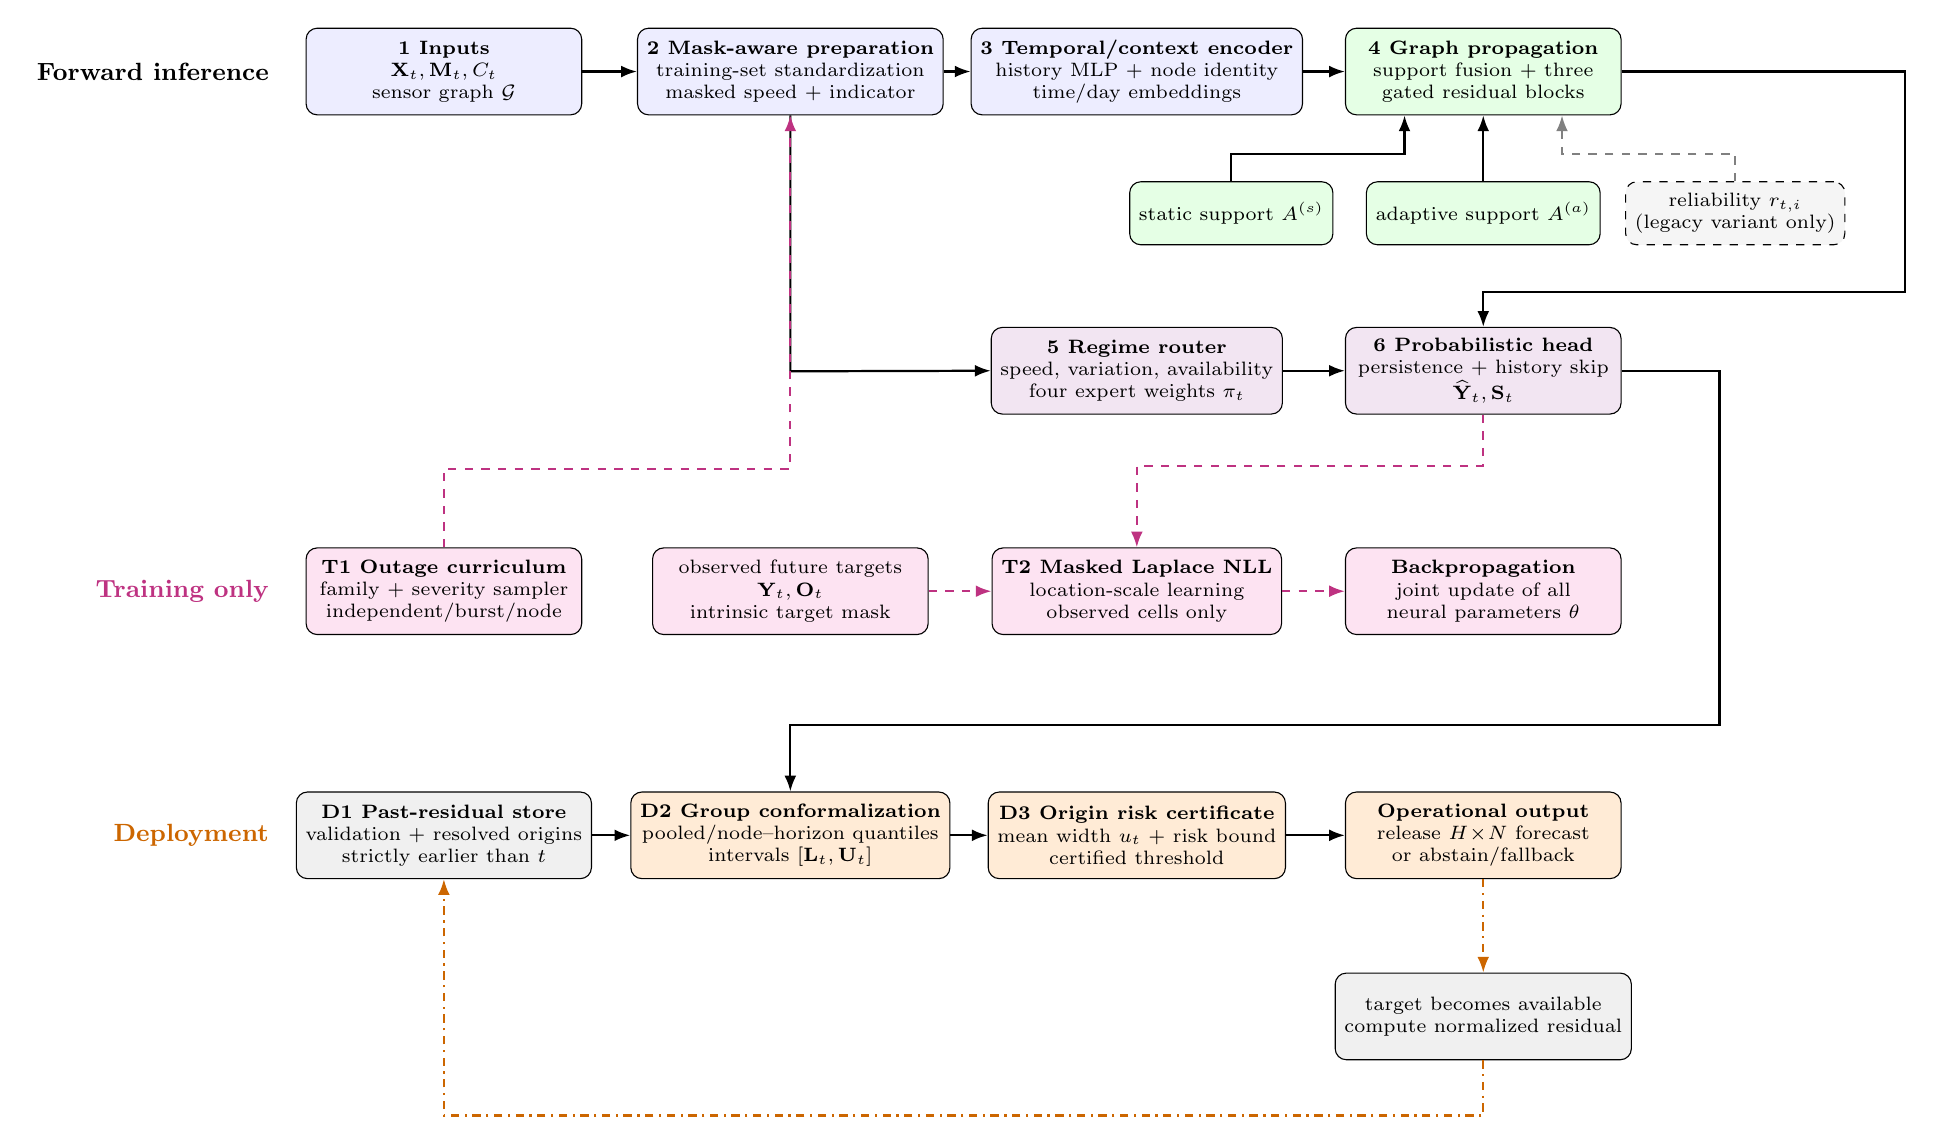
\begin{tikzpicture}[
    x=1cm,y=1cm,
    block/.style={draw,rounded corners,align=center,font=\scriptsize,
      minimum height=11mm,minimum width=35mm,fill=blue!7},
    support/.style={draw,rounded corners,align=center,font=\scriptsize,
      minimum height=8mm,minimum width=25mm,fill=green!10},
    graph/.style={block,fill=green!10},
    prob/.style={block,fill=violet!10},
    decision/.style={block,fill=orange!16},
    train/.style={block,fill=magenta!11},
    memory/.style={block,fill=gray!12},
    flow/.style={-{Latex[length=2mm]},thick},
    trainflow/.style={-{Latex[length=2mm]},thick,dashed,magenta!75!black},
    feedback/.style={-{Latex[length=2mm]},thick,dash dot,orange!80!black},
    label/.style={font=\small\bfseries,anchor=east}
  ]
    \node[label] at (-2.1,0) {Forward inference};
    \node[block] (input) at (0,0) {\textbf{1 Inputs}\\$\mathbf X_t,\mathbf M_t,C_t$\\sensor graph $\mathcal G$};
    \node[block] (mask) at (4.4,0) {\textbf{2 Mask-aware preparation}\\training-set standardization\\masked speed + indicator};
    \node[block] (temporal) at (8.8,0) {\textbf{3 Temporal/context encoder}\\history MLP + node identity\\time/day embeddings};
    \node[graph] (graphblock) at (13.2,0) {\textbf{4 Graph propagation}\\support fusion + three\\gated residual blocks};
    \draw[flow] (input) -- (mask);
    \draw[flow] (mask) -- (temporal);
    \draw[flow] (temporal) -- (graphblock);

    \node[support] (static) at (10.0,-1.8) {static support $A^{(s)}$};
    \node[support] (adaptive) at (13.2,-1.8) {adaptive support $A^{(a)}$};
    \node[support,dashed,fill=gray!8] (reliability) at (16.4,-1.8) {reliability $r_{t,i}$\\(legacy variant only)};
    % Each support uses its own orthogonal channel and a distinct graph-block
    % anchor, preventing the converging arrows from crossing neighboring boxes.
    \draw[flow] (static.north) -- ++(0,0.35)
      -| ([xshift=-10mm]graphblock.south);
    \draw[flow] (adaptive.north) -- (graphblock.south);
    \draw[flow,dashed,gray] (reliability.north) -- ++(0,0.35)
      -| ([xshift=10mm]graphblock.south);

    \node[prob] (router) at (8.8,-3.8) {\textbf{5 Regime router}\\speed, variation, availability\\four expert weights $\pi_t$};
    \node[prob] (head) at (13.2,-3.8) {\textbf{6 Probabilistic head}\\persistence + history skip\\$\widehat{\mathbf Y}_t,\mathbf S_t$};
    % The router reads mask-aware origin statistics, whereas the graph state
    % reaches the prediction head through a separate outer channel.
    \draw[flow] (mask.south) -- ++(0,-3.25) -- (router.west);
    \draw[flow] (graphblock.east) -- ++(3.6,0) -- ++(0,-2.8)
      -| (head.north);
    \draw[flow] (router) -- (head);

    \node[label,magenta!75!black] at (-2.1,-6.6) {Training only};
    \node[train] (augment) at (0,-6.6) {\textbf{T1 Outage curriculum}\\family + severity sampler\\independent/burst/node};
    \node[train] (target) at (4.4,-6.6) {observed future targets\\$\mathbf Y_t,\mathbf O_t$\\intrinsic target mask};
    \node[train] (loss) at (8.8,-6.6) {\textbf{T2 Masked Laplace NLL}\\location-scale learning\\observed cells only};
    \node[train] (update) at (13.2,-6.6) {\textbf{Backpropagation}\\joint update of all\\neural parameters $\theta$};
    \draw[trainflow] (augment.north) -- ++(0,1.0) -| (mask.south);
    \draw[trainflow] (target) -- (loss);
    \draw[trainflow] (head.south) -- ++(0,-0.65) -| (loss.north);
    \draw[trainflow] (loss) -- (update);

    \node[label,orange!80!black] at (-2.1,-9.7) {Deployment};
    \node[memory] (store) at (0,-9.7) {\textbf{D1 Past-residual store}\\validation + resolved origins\\strictly earlier than $t$};
    \node[decision] (conformal) at (4.4,-9.7) {\textbf{D2 Group conformalization}\\pooled/node--horizon quantiles\\intervals $[\mathbf L_t,\mathbf U_t]$};
    \node[decision] (certificate) at (8.8,-9.7) {\textbf{D3 Origin risk certificate}\\mean width $u_t$ + risk bound\\certified threshold};
    \node[decision] (action) at (13.2,-9.7) {\textbf{Operational output}\\release $H\!\times\!N$ forecast\\or abstain/fallback};
    \node[memory] (resolved) at (13.2,-12.0) {target becomes available\\compute normalized residual};
    \draw[flow] (head.east) -- (16.2,-3.8) -- (16.2,-8.3)
      -- (4.4,-8.3) -- (conformal.north);
    \draw[flow] (store) -- (conformal);
    \draw[flow] (conformal) -- (certificate);
    \draw[flow] (certificate) -- (action);
    \draw[feedback] (action) -- (resolved);
    \draw[feedback] (resolved.south) -- ++(0,-0.7) -| (store.south);
  \end{tikzpicture}}
  \caption{Detailed ShiftGuard architecture and leakage-controlled data flow.
  The blue/green/violet forward path produces node--horizon locations and
  scales; the magenta path applies structured-outage training and masked
  probabilistic loss; and the orange deployment path performs prequential
  conformal calibration and origin-level release or abstention. The grey
  dashed reliability input is used only by the legacy variant and is disabled in
  the reference model. Solid arrows
  denote current-origin information, dashed arrows denote training-only
  operations, and dash-dotted arrows denote feedback available only after a
  target has resolved.}
  \label{fig:method-overview}
\end{figure*}
\subsection{Mask-aware encoding and graph propagation}
For a mini-batch of size $B$, the raw model input has shape
$B\times P\times N\times F$, where the first feature is standardized speed and
the remaining channels include the intrinsic observation indicator, time of
day, and day of week. A stress mask $M_t$ is multiplied by the intrinsic
indicator, so naturally absent measurements remain absent. Unobserved speeds
are set to zero only after standardization and are never confused with true
zero speed because the binary mask is supplied separately. For node $i$, the
encoder input is
\begin{equation}
 q_{t,i}=\operatorname{vec}\left([X_{t-P+1:t,i}\odot M_{t,i},M_{t,i}]\right)
 \in\mathbb{R}^{2P}.
\end{equation}
A two-layer GELU multilayer perceptron maps $q_{t,i}$ to a $d=64$ temporal
state. Learned node identity, five-minute time-of-day, and day-of-week
embeddings are added to this state. This direct construction is deliberately
small: it preserves the strong identity-based inductive bias documented by
STID~\cite{shao2022stid} without requiring full spatiotemporal self-attention.

The static support $A^{(s)}$ is a sparse correlation graph built from training
inputs only, keeping each sensor's twelve most positively correlated
neighbors, with self-loops and row normalization. The adaptive support is
\begin{equation}
 A^{(a)}=\operatorname{softmax}\!\left(\operatorname{ReLU}(E_sE_d^\top)\right),
\end{equation}
where $E_s,E_d\in\mathbb{R}^{N\times16}$ are learned source and destination
embeddings. When both supports are enabled, the reference model uses their
row-normalized equal-weight mixture
\begin{equation}
 \widetilde A_{ij}=
 \frac{\tfrac12(A^{(s)}_{ij}+A^{(a)}_{ij})}
 {\sum_k\tfrac12(A^{(s)}_{ik}+A^{(a)}_{ik})+\epsilon}.
\end{equation}
Each of three graph blocks computes a linear message
$m_i=\sum_j\widetilde A_{ij}W_mz_j$ and a gate $g_i=\sigma(W_g[z_i,m_i,1])$. The
update is a normalized residual mixture of $m_i$ and $z_i$. Residual
connections preserve local information when neighbors are missing, while
dropout regularizes the exchanged messages. Missingness therefore reaches the
model through the mask channel of $q_{t,i}$ and through the router statistics,
not through the graph weights.

The first version of ShiftGuard additionally weighted each sender by its
average input availability $r_{t,j}=P^{-1}\sum_{p=1}^{P}M_{t-p+1,j}$, replacing
$\widetilde A_{ij}$ by
$\widetilde A_{t,ij}\propto\tfrac12(A^{(s)}_{ij}+A^{(a)}_{ij})r_{t,j}$ and the
constant gate input by $r_{t,i}$, so that a sender with no usable history
contributed little to its neighbors. Section~\ref{sec:reference-selection}
explains why this \emph{reliability weighting} is disabled in the reference
model; the legacy variant is retained as an ablation.

\subsection{Regime routing and probabilistic head}
Four global statistics summarize the current origin: mean speed, speed standard
deviation, mean absolute first difference, and mean sensor availability. A
two-layer router converts them to weights
$\pi_t=\operatorname{softmax}(f_{\mathrm{route}}(c_t))$ over $K=4$ compact
output experts. Expert $k$ maps every node state to $H$ median residuals and $H$
positive scales. The combined outputs are
\begin{align}
 \hat Y_t &= X_{t,\mathrm{last}}+
 W_{\mathrm{skip}}X_{t-P+1:t}+\sum_{k=1}^{K}\pi_{t,k}\mu_{t,k},\\
 S_t &= \sum_{k=1}^{K}\pi_{t,k}
 \left[\operatorname{softplus}(s_{t,k})+10^{-4}\right].
\end{align}
The last-observation term makes persistence an easy initial solution, while the
zero-initialized history projection learns a direct multi-horizon correction.
The model has 89,012 parameters for METR-LA and 100,340 for PEMS-BAY. The router
is retained in the evaluated full system for preregistration fidelity, but the
ablation results later show that it is not the source of the robustness gain.

The location and scale are trained with the Laplace negative log likelihood
over observed target cells,
\begin{equation}
 \mathcal{L}_{\mathrm{Lap}}=
 \frac{1}{|\Omega|}\sum_{(h,i)\in\Omega}
 \left(\frac{|Y_{t,h,i}-\hat Y_{t,h,i}|}{S_{t,h,i}}+
 \log(2S_{t,h,i})\right),
\end{equation}
where $\Omega$ excludes unavailable ground truth. AdamW, gradient clipping, and
validation early stopping optimize this objective. The probabilistic scale is
not treated as calibrated by construction; it becomes a normalization factor
for the conformal residual score.

\subsection{Structured-outage curriculum}
At every training batch, a seeded generator samples one of three outage
families and a severity $r\sim\mathcal{U}(0,0.4)$. Independent loss removes
individual sensor--time cells with probability $r$. Burst loss selects each
sensor with probability $r$ and masks a random suffix of its history. Whole-node
loss removes a random $r$ fraction of sensors for the full input window. Masked
speeds are set to zero in standardized units, and the mask is supplied to the
model. Contiguous-region and high-degree hub outages are never generated during
training; they are held-out test geometries that assess whether the
augmentation generalizes to unseen correlated failure. The confirmatory test
masks are generated once, stored, and reused by every model and seed, so
differences cannot arise from different failure samples. Nothing in the
curriculum depends on the ShiftGuard architecture, which allows the same
procedure to be applied unchanged to the baselines in
Section~\ref{sec:fair-comparison}. The no-augmentation and independent-only
variants test the mechanism within ShiftGuard.

\subsection{Conformal risk control}
\label{sec:evidence-gating-calibration-anchor}
For a resolved calibration origin $u$, node--horizon nonconformity is
\begin{equation}
 R_{u,h,i}=\frac{|Y_{u,h,i}-\hat Y_{u,h,i}|}{S_{u,h,i}}.
\end{equation}
Before predicting origin $t$, the rolling calibrator contains only
$\{R_u:u<t\}$. It estimates the finite-sample conformal quantile separately for
every $(h,i)$ group and shrinks small groups toward the pooled quantile. If
$n_{h,i}$ usable scores occur in the rolling window and $\tau$ is the shrinkage
constant, the effective radius is based on
$w_{h,i}q_{h,i}+(1-w_{h,i})q_{\mathrm{global}}$, with
$w_{h,i}=n_{h,i}/(n_{h,i}+\tau)$. The interval is
\begin{equation}
 [L_{t,h,i},U_{t,h,i}]=
 [\hat Y_{t,h,i}-q_{t,h,i}S_{t,h,i},
  \hat Y_{t,h,i}+q_{t,h,i}S_{t,h,i}].
\end{equation}
Rolling updates allow the scale to react after distribution changes, but they
do not convert dependent traffic into an exchangeable sample. We therefore
report marginal, worst-node--horizon, and worst-regime empirical coverage and
avoid a prospective conditional-coverage claim.

Selection operates at the forecast-origin level. Define realized operational
error and uncertainty score as
\begin{equation}
 e_t=(HN)^{-1}\sum_{h,i}|Y_{t,h,i}-\hat Y_{t,h,i}|,
 \qquad
 u_t=(HN)^{-1}\sum_{h,i}(U_{t,h,i}-L_{t,h,i}).
\end{equation}
Candidate thresholds are quantiles of $u_t$ from even-indexed past origins.
For each threshold, odd-indexed past origins estimate the Bernoulli failure
indicator $\mathbb{1}\{e_t>5\ \mathrm{mph}\}$ among accepted forecasts. The
controller chooses the largest retained fraction whose Bonferroni-corrected
Clopper--Pearson upper confidence bound is at most the registered 10\% risk
limit at familywise $\delta=0.05$. If no candidate is certified, it abstains.
Sorting all origins by $u_t$ also yields the risk--coverage curve and its area
(AURC); lower AURC means that uncertainty ranks harmful forecasts more
effectively.

At deployment, the sequence is therefore: (1) ingest the latest speed and
availability window; (2) compute point and scale tensors; (3) form intervals
from past residuals; (4) compare mean width with the certified threshold; (5)
release or withhold the full tensor; and (6) after its target resolves, append
the new residual to the rolling calibration store. This ordered pipeline is the
central leakage-control invariant of the system.

\subsection{Evidence gating}
\label{sec:evidence-gating}
A forecast for a sensor that has stopped reporting cannot rest on that sensor's
recent history. Evidence gating therefore assigns each sensor at each origin to a
freshness level: fresh if it reported at the origin, recent if its last report
was 1--5 steps earlier, stale if it was 6 or more steps earlier, and blind if it
reported nothing in the input window. For each level and horizon, the output is
$w\widehat{Y}+(1-w)F$, where $F$ is a time-of-week historical profile computed
from training data only and $w\in\{0,0.05,\dots,1\}$ minimizes validation MAE
under simulated validation outages drawn with dedicated seeds.

Conformal quantiles are computed per freshness level and horizon in the same
block-prequential manner as Section~\ref{sec:evidence-gating-calibration-anchor},
pooling levels with fewer than 50 residuals. Silent sensors never produce
outcomes in deployment, so their residuals cannot be observed directly.
\emph{Shadow blinding} obtains them from working sensors: a random 15\% are
hidden for the whole input window and a further 15\% for a random suffix of it,
the model is rerun, and the resulting residuals are scored once those sensors'
readings arrive. No test outcome from a failed sensor enters calibration.

\section{Experimental design}
\subsection{Datasets and leakage control}
\textbf{METR-LA.} The Los Angeles benchmark contains speed readings from 207
loop detectors on metropolitan-area freeways. The checksum-verified file used
here spans 1 March to 27 June 2012 and contains 34,272 five-minute timestamps,
equivalent to 119 days. After interpreting non-finite and non-positive readings
as unavailable, 8.109\% of sensor--time cells are missing. The observed mean is
58.460 mph and the standard deviation is 13.024 mph. METR-LA contains a
meaningful mixture of operating conditions: 4.35\% of valid readings are below
25 mph, 72.60\% exceed 55 mph, and 14.09\% of consecutive sensor readings change
by more than 5 mph. Its pooled autocorrelation is 0.942 at one five-minute lag,
0.715 at one hour, 0.627 at one day, and 0.709 at one week. These statistics
indicate strong persistence and periodicity but also substantially more native
missingness and volatility than PEMS-BAY.

\textbf{PEMS-BAY.} The Bay Area benchmark contains 325 freeway sensors and
52,116 five-minute timestamps from 1 January to 30 June 2017, or 181 days. Its
native missing fraction after the same validity rule is only 0.003\%. Mean speed
is 62.621 mph with a 9.588 mph standard deviation. Readings below 25 mph account
for 1.92\%, while 90.32\% exceed 55 mph; only 2.30\% of consecutive sensor
measurements change by more than 5 mph. Autocorrelation is 0.983 at five
minutes, 0.731 at one hour, 0.681 at one day, and 0.780 at one week. PEMS-BAY is
therefore larger, cleaner, and more strongly persistent. Reporting both
datasets is important because robustness that holds only on METR-LA could be an
artifact of its existing missingness, while robustness that holds only on
PEMS-BAY might not transfer to a noisier network.

\textbf{Graph and feature construction.} To avoid reliance on incompatible
external graph files, the static support is reconstructed from the training
input only. Pairwise sensor correlations are computed over training histories;
for every node, the 12 strongest non-negative correlations are retained. The
same support is supplied to all graph-based models and to the region/hub outage
generators. Each window contains standardized speed, a native-availability
indicator, normalized five-minute time of day, and normalized day of week.
Only the speed channel is forecast. This correlation graph is a reproducible
proxy, not a claim to recover true road causality, and its limitations are
discussed in Section~7.

\textbf{Chronological splits and windows.} Raw timestamps are partitioned
before windowing into 70\% training, 10\% validation, and 20\% test segments.
For METR-LA this produces 23,967 training, 3,416 validation, and 6,844 test
forecast origins; for PEMS-BAY it produces 36,458, 5,200, and 10,413 origins.
Twelve historical samples (60 minutes) directly predict the next twelve
samples (60 minutes). Validation and test inputs may use the immediately
preceding 60 minutes as context, but every target lies inside its own split.
Consequently, a target never crosses backward into the training or validation
block.

\textbf{Missingness and normalization.} Per-sensor mean and standard deviation
are fitted only on observed training values. Missing input speed is replaced by
the training mean before standardization, becoming zero in normalized space,
and the mask channel preserves its unavailable status. Missing targets are
excluded from loss and metrics. All reported MAE and RMSE values are inverse
transformed to mph. Test data are never used for normalization, early stopping,
hyperparameter selection, conformal initialization, or selection-threshold
construction. Dataset diagnostics in Table~\ref{tab:datasets} are generated
directly from the raw files rather than copied from secondary papers.
\begin{table*}[t]
  \centering
  \caption{Dataset diagnostics computed from checksum-verified raw files.
  Speed is in miles per hour; correlations use observed values at 5-minute and
  one-day lags.}
  \label{tab:datasets}
  \resizebox{\textwidth}{!}{\begin{tabular}{lrrrrrrr}
\toprule
Dataset & Timestamps & Sensors & Missing (pct.) & Mean speed & Std. speed & Lag-1 corr. & Lag-288 corr. \\
\midrule
METR-LA & 34272 & 207 & 8.109 & 58.460 & 13.024 & 0.942 & 0.627 \\
PEMS-BAY & 52116 & 325 & 0.003 & 62.621 & 9.588 & 0.983 & 0.681 \\
\bottomrule
\end{tabular}
}
\end{table*}

\subsection{Reference-model selection}
\label{sec:reference-selection}
The first version of ShiftGuard included reliability-weighted propagation.
Its test-set ablations showed that disabling this weighting reduced stressed
MAE on both datasets (Table~\ref{tab:ablation-legacy}). Choosing the reported
model from those test results would bias its evaluation, so the reference model
is selected on validation data only. Each ShiftGuard variant is scored on the
validation split under the four outage families at 30\% severity, using masks
drawn with a dedicated seed that is never used for test masks, and the variant
with the lowest stressed MAE averaged over both datasets is selected. The
no-reliability variant obtains 2.953 and 1.907 mph on METR-LA and PEMS-BAY
(mean 2.430), compared with 2.985 and 1.893 mph for adaptive-graph-only
propagation (mean 2.439), 3.018 and 1.941 mph without the router, and 3.044 and
1.965 mph for the legacy model. The margin over adaptive-graph-only propagation
is small, and that variant is better on PEMS-BAY; we therefore treat the two as
near-equivalent and report the adaptive-graph variant among the ablations.
All results labelled ShiftGuard refer to this reference model. Its checkpoints
are the five seeds originally trained for the no-reliability ablation, so no
model was retrained after test results were seen. Ablations of the reference
model are newly trained under the unchanged protocol.

\subsection{Baselines}
Locally reproduced baselines include historical average, persistence, ridge AR,
linear, MLP/GRU, STGCN, DCRNN, Graph WaveNet, AGCRN, STID, and a faithful
STAEformer configuration. Compatible open implementations of
recent methods are added after preprocessing and license audits. Reported SOTA
values appear in a separate contextual table and are never used for significance
claims. The recurrent and graph baselines are protocol-matched compact
reproductions, not claims of bitwise equivalence to their authors' code; a
model-by-model deviation audit accompanies the repository.

Standard baselines are trained on fully observed inputs and emit only a point
forecast. A comparison against them confounds architecture with training
distribution and with the availability of a learned scale. We therefore add two
recipe-matched variants for STID, DCRNN, Graph WaveNet, AGCRN, and STAEformer.
The \emph{outage-augmented} variant uses the identical mask generator,
severity distribution, and input zeroing as ShiftGuard. The
\emph{outage-augmented Laplace} variant additionally doubles the width of the
baseline's final output layer to emit a median and a softplus scale and is
trained with the same Laplace negative log-likelihood. Backbones,
hyperparameters, optimizer, early stopping, seeds, test masks, calibration, and
the risk controller are otherwise unchanged. Recipe-matched variants enter the
recipe-versus-architecture analysis and are excluded from the canonical clean
accuracy table.
\begin{table*}[t]
  \centering
  \caption{Literature-reported point accuracy for context only. Protocol and
  implementation differences prohibit direct significance comparisons with
  locally reproduced results.}
  \label{tab:reported-context}
  \resizebox{\textwidth}{!}{\begin{tabular}{llllll}
\toprule
Dataset & Model & MAE at 15 min & MAE at 30 min & MAE at 60 min & Average MAE \\
\midrule
METR-LA & DCRNN & 2.77 & 3.15 & 3.60 & -- \\
METR-LA & Graph WaveNet & 2.69 & 3.08 & 3.51 & -- \\
METR-LA & STAEformer & 2.65 & 2.97 & 3.34 & -- \\
METR-LA & TESTAM & -- & -- & -- & 2.93 \\
PEMS-BAY & DCRNN & 1.38 & 1.74 & 2.07 & -- \\
PEMS-BAY & Graph WaveNet & 1.30 & 1.63 & 1.99 & -- \\
PEMS-BAY & STAEformer & 1.31 & 1.62 & 1.88 & -- \\
PEMS-BAY & TESTAM & -- & -- & -- & 1.53 \\
\bottomrule
\end{tabular}
}
\end{table*}

\subsection{Deployment-feasible protocol}
\label{sec:deployment-protocol}
In this protocol, an outage is a property of a sensor at a timestamp, so
consecutive forecast origins see the same failure and a failed sensor's future
readings are unavailable. Six primary scenarios are evaluated. \emph{Native} adds
no outage. \emph{Trace-x1} and \emph{trace-x2} replay real availability from the
METR-LA training period at one or two superposed time offsets, preserving
co-failures. \emph{Sensor-s30} simulates independent alternating-renewal failures
of 30\% of cells, using empirical METR-LA down durations. \emph{Region-s30} and
\emph{hub-s15} use episodes of at least one hour that remove a correlated cluster
of 15\% of sensors, or 15\% of sensors drawn from the top 30\% by degree. Hub
severity is 15\% because 30\% is unreachable under that pool, so it is not
matched to the other families. PEMS-BAY has almost no native missingness, so its
traces and durations are transplanted from METR-LA by sampling sensor columns,
which preserves failure timing but not physical sensor identity. Models are
compared on identical timelines for each seed.

Three calibration arms differ in what the calibrator may read: \emph{oracle
feedback} reads all outcomes and is an upper bound, \emph{feasible} reads only
what working sensors reported, and \emph{feasible-thinned} also restricts the
risk certificate to origins with non-overlapping targets. All scores use withheld
truth, including at failed sensors. Abstention releases the training-only
historical profile, and is compared with always releasing, with random abstention
at the same rate, and with an oracle. Metrics include MAE overall and at blind
sensors; coverage overall, at blind sensors, and by worst group; retention and
failure among released forecasts; excess AURC; failure AUROC; and the share of
days over the risk limit. Intervals use crossed seed--day bootstrapping.

Evidence gating was motivated by a test-set pilot on METR-LA seed~1, which is
therefore exploratory. The gating claims rest on PEMS-BAY and the other four
METR-LA seeds, and nothing was tuned after the hypotheses were recorded:
H1, gating lowers MAE at blind sensors relative to the unblended model;
H2, gating does not raise fresh-sensor MAE by more than 1\%;
H3, shadow calibration brings blind-cell coverage closer to 0.90 than
node--horizon calibration with feasible feedback;
H4, network-level abstention to the fallback lowers MAE relative to always
releasing.

\subsection{Legacy stress protocol and metrics}
\label{sec:legacy-protocol}
Our first evaluation crossed clean, independent, temporal-burst,
contiguous-region, and high-degree hub outages at 10--50\% severity with
free-flow, stable intermediate, and transition regimes. No origin in either test
set meets the congested-regime definition, so no claim is made about congested
traffic. A subsequent audit found three further defects: window-level masks can
disagree across overlapping windows, region and hub outages last the entire test
block, and calibration reads outcomes from failed sensors. Interval and selection
results under this protocol are therefore optimistic and are reported only for
continuity. Metrics include horizon-specific and average MAE, RMSE, MAPE;
degradation and worst-regime MAE; coverage, width, Winkler score and worst-group
coverage; AURC and selective MAE; parameters, FLOPs, latency, peak memory, and
training time. Results use five seeds and paired bootstrap confidence
intervals.

The confirmatory environment is captured automatically, including Python and
package versions, CUDA build, GPU, and driver. Runs use PyTorch 2.13.0 with CUDA
13.0 on an NVIDIA GeForce RTX 5060 Laptop GPU; the generated environment
manifest is retained with the result artifacts.

\section{Results}
\subsection{Canonical accuracy}
Table~\ref{tab:local-headline} is generated exclusively from local experiment
artifacts. A stochastic model enters the confirmatory table only after all five
registered seeds complete; partial runs are omitted.
\begin{table*}[t]
  \centering
  \caption{Locally reproduced canonical-test results. Empty uncertainty cells
  indicate that only one deterministic run is applicable or currently complete.}
  \label{tab:local-headline}
  \resizebox{\textwidth}{!}{\begin{tabular}{llrlrrrrr}
\toprule
Dataset & Model & MAE & SD & RMSE & MAPE (pct.) & Parameters & Train (s) & Seeds \\
\midrule
METR-LA & ShiftGuard & 3.004 & 0.007 & 6.018 & 8.340 & 89012 & 985.362 & 5 \\
METR-LA & STAEformer & 3.032 & 0.008 & 6.178 & 8.362 & 1258932 & 4554.221 & 5 \\
METR-LA & DCRNN & 3.247 & 0.010 & 6.380 & 9.133 & 63372 & 1002.598 & 5 \\
METR-LA & STID & 3.273 & 0.015 & 6.603 & 9.558 & 41996 & 90.004 & 5 \\
METR-LA & Graph WaveNet & 3.285 & 0.008 & 6.451 & 9.205 & 22744 & 749.354 & 5 \\
METR-LA & AGCRN & 3.343 & 0.010 & 6.576 & 9.494 & 16764 & 492.095 & 5 \\
METR-LA & GRU & 3.761 & 0.002 & 7.628 & 10.878 & 13644 & 464.916 & 5 \\
METR-LA & MLP & 3.798 & 0.002 & 7.662 & 11.032 & 5772 & 68.023 & 5 \\
METR-LA & STGCN & 3.899 & 0.013 & 7.187 & 11.365 & 17548 & 374.899 & 5 \\
METR-LA & Linear & 3.982 & 0.001 & 7.728 & 11.589 & 156 & 48.049 & 5 \\
METR-LA & Historical average & 4.189 & -- & 7.856 & 13.044 & 0 & 0.000 & 1 \\
METR-LA & Persistence & 4.244 & -- & 8.154 & 11.052 & 0 & 0.000 & 1 \\
METR-LA & Ridge AR & 4.294 & -- & 7.595 & 12.727 & 324 & 0.093 & 1 \\
PEMS-BAY & STAEformer & 1.577 & 0.006 & 3.650 & 3.613 & 1372212 & 13896.209 & 5 \\
PEMS-BAY & ShiftGuard & 1.590 & 0.004 & 3.574 & 3.665 & 100340 & 1674.960 & 5 \\
PEMS-BAY & STID & 1.664 & 0.004 & 3.739 & 3.822 & 49548 & 199.245 & 5 \\
PEMS-BAY & DCRNN & 1.683 & 0.005 & 3.779 & 3.900 & 63372 & 2888.655 & 5 \\
PEMS-BAY & Graph WaveNet & 1.720 & 0.005 & 3.770 & 3.934 & 25104 & 1830.569 & 5 \\
PEMS-BAY & AGCRN & 1.731 & 0.004 & 3.849 & 4.016 & 18652 & 1338.461 & 5 \\
PEMS-BAY & GRU & 1.955 & 0.001 & 4.619 & 4.566 & 13644 & 1081.630 & 5 \\
PEMS-BAY & MLP & 1.969 & 0.004 & 4.648 & 4.569 & 5772 & 169.266 & 5 \\
PEMS-BAY & Linear & 2.130 & 0.001 & 4.955 & 4.808 & 156 & 71.894 & 5 \\
PEMS-BAY & Persistence & 2.171 & -- & 5.125 & 4.671 & 0 & 0.000 & 1 \\
PEMS-BAY & Ridge AR & 2.302 & -- & 4.831 & 5.371 & 324 & 0.086 & 1 \\
PEMS-BAY & STGCN & 2.506 & 0.005 & 4.873 & 5.918 & 17548 & 903.628 & 5 \\
PEMS-BAY & Historical average & 2.630 & -- & 5.228 & 6.176 & 0 & 0.000 & 1 \\
\bottomrule
\end{tabular}
}
\end{table*}

\begin{figure*}[t]
  \centering
  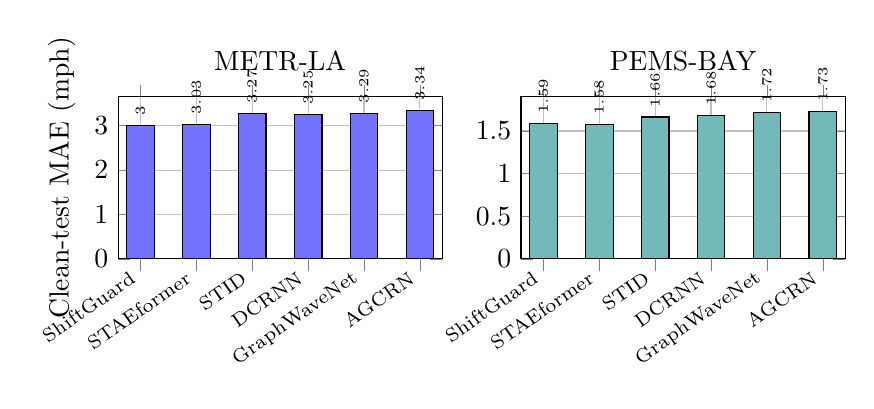
\begin{tikzpicture}
    \begin{groupplot}[
      group style={group size=2 by 1,horizontal sep=1.0cm},
      ybar,width=0.47\textwidth,height=0.30\textwidth,
      symbolic x coords={ShiftGuard,STAEformer,STID,DCRNN,GraphWaveNet,AGCRN},
      xtick=data,x tick label style={rotate=35,anchor=east,font=\scriptsize},
      nodes near coords,nodes near coords style={font=\tiny,rotate=90,anchor=west},
      ymin=0,grid=major,enlarge x limits=0.08]
      \nextgroupplot[title={METR-LA},ylabel={Clean-test MAE (mph)},ymax=3.65]
        \addplot[fill=blue!55] coordinates {
          (ShiftGuard,3.004) (STAEformer,3.032) (STID,3.273)
          (DCRNN,3.247) (GraphWaveNet,3.285) (AGCRN,3.343)};
      \nextgroupplot[title={PEMS-BAY},ymax=1.90]
        \addplot[fill=teal!55] coordinates {
          (ShiftGuard,1.590) (STAEformer,1.577) (STID,1.664)
          (DCRNN,1.683) (GraphWaveNet,1.720) (AGCRN,1.731)};
    \end{groupplot}
  \end{tikzpicture}
  \caption{Clean-test comparison chart for the strongest locally reproduced
  neural baselines. ShiftGuard is slightly more accurate than STAEformer on
  METR-LA but does not achieve clean-data SOTA on PEMS-BAY.}
  \label{fig:clean-comparison}
\end{figure*}

Figure~\ref{fig:clean-comparison} makes the clean-data ranking explicit. On
METR-LA, ShiftGuard improves on STAEformer by 0.028 mph in pooled MAE (3.004
versus 3.032), and both improve on the next group of graph baselines. On
PEMS-BAY, STAEformer leads ShiftGuard by 0.013 mph; STID and DCRNN remain close
behind. ShiftGuard has the lower RMSE of the two leading methods on both datasets
(6.018 versus 6.178 and 3.574 versus 3.651), suggesting fewer large residuals
even where its mean absolute error is slightly higher. This observation is
descriptive; the paired origin-level analysis below determines inferential
claims.

Paired inference uses non-overlapping daily blocks of forecast origins. The
reported confidence interval is a crossed seed--day paired-bootstrap interval for
$\Delta\mathrm{MAE}=\mathrm{MAE}_{\text{ShiftGuard}}-
\mathrm{MAE}_{\text{comparator}}$; both seeds and chronological daily blocks
are resampled. Wilcoxon tests operate on paired daily-block differences averaged
over seeds and are Holm corrected across the displayed comparisons.
\begin{table*}[t]
  \centering
  \caption{Paired daily-block statistical comparison. Negative $\Delta$MAE
  favors ShiftGuard.}
  \label{tab:paired-statistics}
  \resizebox{\textwidth}{!}{\begin{tabular}{llrrrrl}
\toprule
Dataset & Comparator & Delta MAE & CI low & CI high & Improvement (pct.) & Holm p \\
\midrule
METR-LA & agcrn & -0.3455 & -0.3895 & -0.3064 & 10.2632 & $<0.0001$ \\
METR-LA & dcrnn & -0.2482 & -0.2931 & -0.2212 & 7.5935 & $<0.0001$ \\
METR-LA & graphwavenet & -0.2853 & -0.3190 & -0.2489 & 8.6305 & $<0.0001$ \\
METR-LA & gru & -0.7587 & -0.8455 & -0.6425 & 20.0732 & $<0.0001$ \\
METR-LA & historical average & -1.1805 & -1.3435 & -1.0882 & 28.0974 & $<0.0001$ \\
METR-LA & linear & -0.9808 & -1.0791 & -0.8554 & 24.5096 & $<0.0001$ \\
METR-LA & mlp & -0.8001 & -0.8949 & -0.6988 & 20.9402 & $<0.0001$ \\
METR-LA & persistence & -1.2433 & -1.3269 & -1.1294 & 29.1573 & $<0.0001$ \\
METR-LA & ridge ar & -1.2917 & -1.3804 & -1.1741 & 29.9523 & $<0.0001$ \\
METR-LA & shiftguard & -0.0294 & -0.0467 & -0.0050 & 0.9654 & 0.0015 \\
METR-LA & staeformer & -0.0301 & -0.0500 & -0.0127 & 0.9879 & 0.0034 \\
METR-LA & stgcn & -0.8964 & -0.9647 & -0.8330 & 22.8841 & $<0.0001$ \\
METR-LA & stid & -0.2726 & -0.3289 & -0.2371 & 8.2758 & $<0.0001$ \\
PEMS-BAY & agcrn & -0.1404 & -0.1617 & -0.1155 & 8.1129 & $<0.0001$ \\
PEMS-BAY & dcrnn & -0.0925 & -0.1099 & -0.0714 & 5.4987 & $<0.0001$ \\
PEMS-BAY & graphwavenet & -0.1295 & -0.1461 & -0.1088 & 7.5298 & $<0.0001$ \\
PEMS-BAY & gru & -0.3649 & -0.4277 & -0.2873 & 18.6632 & $<0.0001$ \\
PEMS-BAY & historical average & -1.0402 & -1.2105 & -0.9078 & 39.5471 & $<0.0001$ \\
PEMS-BAY & linear & -0.5398 & -0.6261 & -0.4310 & 25.3447 & $<0.0001$ \\
PEMS-BAY & mlp & -0.3790 & -0.4446 & -0.2973 & 19.2481 & $<0.0001$ \\
PEMS-BAY & persistence & -0.5804 & -0.6668 & -0.4730 & 26.7419 & $<0.0001$ \\
PEMS-BAY & ridge ar & -0.7122 & -0.8052 & -0.5949 & 30.9342 & $<0.0001$ \\
PEMS-BAY & shiftguard & -0.0140 & -0.0204 & -0.0075 & 0.8725 & $<0.0001$ \\
PEMS-BAY & staeformer & 0.0129 & 0.0034 & 0.0218 & -0.8190 & 0.0040 \\
PEMS-BAY & stgcn & -0.9157 & -0.9754 & -0.8409 & 36.5442 & $<0.0001$ \\
PEMS-BAY & stid & -0.0739 & -0.1018 & -0.0513 & 4.4412 & $<0.0001$ \\
\bottomrule
\end{tabular}
}
\end{table*}

On METR-LA, ShiftGuard is more accurate than the local STAEformer on the clean
test: the origin-weighted MAE difference is $-0.030$ mph (crossed-bootstrap
95\% interval $[-0.050,\,-0.013]$ mph; Holm-adjusted $p=0.0034$). The effect is
small, about 1\% of MAE, and this statistical estimand weights forecast origins
equally, whereas the canonical table pools observed node--horizon errors. On
PEMS-BAY, STAEformer is better: the origin-weighted difference is $0.013$ mph,
with a 95\% interval $[0.003,0.022]$ and Holm-adjusted $p=0.0040$. ShiftGuard
is therefore not presented as a new clean-data point-forecasting SOTA, and the
proposed reliability contribution requires independent support from the
registered outage and selective-prediction experiments.

\subsection{Deployment-feasible results}
\label{sec:deployment-results}
\pending{Generate tables from scripts/aggregate\_deployment.py once all seeds
finish. Report: (i) MAE, coverage, retention, and failure for each model and
scenario with feasible calibration; (ii) the policy value of abstaining to the
fallback against random and oracle abstention; (iii) the gap between the oracle
and feasible arms; (iv) H1--H4, with failed hypotheses reported as failed, using
the gating-confirmatory seeds only.}

\subsection{Legacy stress comparison}
These results use the protocol of Section~\ref{sec:legacy-protocol}, whose defects
make its interval and selection results optimistic. They are not the basis of
our claims. Table~\ref{tab:stress-main} averages the registered 30\% non-clean outage
families; all family-by-rate results remain available in machine-readable
artifacts.
\begin{table*}[t]
  \centering
  \caption{Compound-shift point, interval, and selective reliability. PI is the
  90\% prediction interval; failure denotes accepted forecasts exceeding the
  registered 5 mph error tolerance. Worst node--horizon (N--H) and regime
  coverage are reported for ShiftGuard and its strongest local comparator.}
  \label{tab:stress-main}
  \resizebox{\textwidth}{!}{\begin{tabular}{llrrrrrrrr}
\toprule
Dataset & Model & MAE & PI coverage & Worst N-H cov. & Worst regime cov. & AURC & Retained & Failure rate & Seeds \\
\midrule
METR-LA & AGCRN & 4.729 & 0.891 & -- & -- & 4.950 & 0.000 & -- & 5 \\
METR-LA & DCRNN & 4.629 & 0.891 & -- & -- & 4.791 & 0.000 & -- & 5 \\
METR-LA & Graph WaveNet & 4.895 & 0.890 & -- & -- & 5.125 & 0.000 & -- & 5 \\
METR-LA & GRU & 4.919 & 0.893 & -- & -- & 5.181 & 0.000 & -- & 5 \\
METR-LA & Linear & 5.109 & 0.894 & -- & -- & 5.356 & 0.000 & -- & 5 \\
METR-LA & MLP & 5.054 & 0.893 & -- & -- & 5.301 & 0.000 & -- & 5 \\
METR-LA & Persistence & 5.478 & 0.895 & -- & -- & 5.703 & 0.000 & -- & 5 \\
METR-LA & ShiftGuard & 3.399 & 0.898 & 0.831 & 0.882 & 2.400 & 0.864 & 0.078 & 5 \\
METR-LA & STAEformer & 3.760 & 0.894 & 0.816 & 0.809 & 3.873 & 0.055 & 0.235 & 5 \\
METR-LA & STGCN & 5.309 & 0.893 & -- & -- & 5.536 & 0.000 & -- & 5 \\
METR-LA & STID & 4.092 & 0.894 & -- & -- & 4.256 & 0.000 & -- & 5 \\
PEMS-BAY & AGCRN & 3.073 & 0.890 & -- & -- & 2.952 & 0.174 & 0.115 & 5 \\
PEMS-BAY & DCRNN & 2.956 & 0.889 & -- & -- & 2.844 & 0.183 & 0.109 & 5 \\
PEMS-BAY & Graph WaveNet & 2.928 & 0.889 & -- & -- & 2.824 & 0.203 & 0.102 & 5 \\
PEMS-BAY & GRU & 3.109 & 0.893 & -- & -- & 3.074 & 0.167 & 0.126 & 5 \\
PEMS-BAY & Linear & 3.199 & 0.894 & -- & -- & 3.221 & 0.077 & 0.203 & 5 \\
PEMS-BAY & MLP & 3.135 & 0.893 & -- & -- & 3.105 & 0.167 & 0.127 & 5 \\
PEMS-BAY & Persistence & 3.283 & 0.894 & -- & -- & 3.268 & 0.001 & 0.267 & 5 \\
PEMS-BAY & ShiftGuard & 1.948 & 0.898 & 0.851 & 0.887 & 1.130 & 0.978 & 0.020 & 5 \\
PEMS-BAY & STAEformer & 2.516 & 0.890 & 0.834 & 0.701 & 2.402 & 0.442 & 0.085 & 5 \\
PEMS-BAY & STGCN & 3.857 & 0.893 & -- & -- & 3.752 & 0.073 & 0.221 & 5 \\
PEMS-BAY & STID & 2.649 & 0.891 & -- & -- & 2.544 & 0.209 & 0.099 & 5 \\
\bottomrule
\end{tabular}
}
\end{table*}

Across independent, burst, region, and hub outages at 10, 20, 30, 40, and
50\%, the mean ShiftGuard--STAEformer MAE difference is $-0.476$ mph on
METR-LA (crossed seed--scenario 95\% interval $[-0.594,-0.366]$) and $-0.617$
mph on PEMS-BAY ($[-0.745,-0.491]$). Corresponding AURC differences are
$-1.51$ and $-1.28$. At 30\%, worst node--horizon coverage is 0.830 versus
0.816 on METR-LA and 0.852 versus 0.834 on PEMS-BAY; worst-regime coverage is
0.887 versus 0.809 and 0.876 versus 0.701. Seed-level Wilcoxon tests cannot
reject after ten-comparison Holm
correction ($p_{\mathrm{Holm}}=0.625$), whose attainable resolution is limited
by five seeds; we therefore report the hierarchical intervals and effects but
do not claim adjusted rank-test significance.

Severity sensitivity provides stronger evidence than a single 30\% slice. On
METR-LA, the ShiftGuard advantage over STAEformer grows from 0.181 mph at 10\%
outage to 0.727 mph at 50\%; on PEMS-BAY it grows from 0.254 to 0.940 mph.
Relative to STAEformer, the 50\%-severity reductions are approximately 17.2\%
and 30.9\%. The curves remain ordered at every tested severity, so the aggregate
effect is not driven by one operating point. STID is consistently less robust
than both leading models, showing that a compact identity-based architecture
alone is insufficient; exposure to structured partial observations is the
critical distinction.

\begin{figure*}[t]
  \centering
  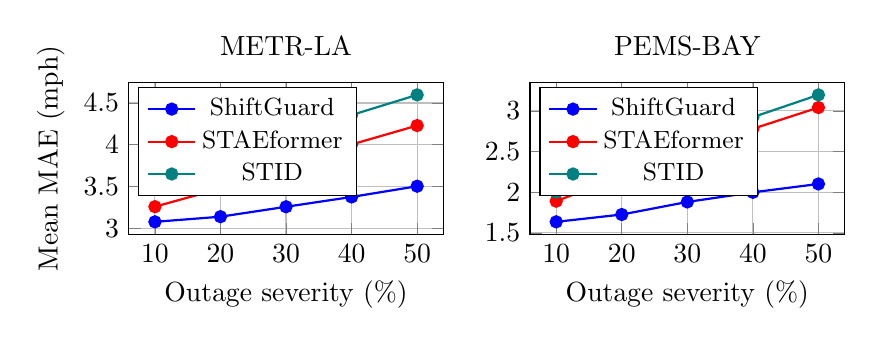
\begin{tikzpicture}
    \begin{groupplot}[
      group style={group size=2 by 1,horizontal sep=1.1cm},
      width=0.46\textwidth,height=0.29\textwidth,
      xlabel={Outage severity (\%)},
      xtick={10,20,30,40,50},grid=major,legend style={font=\small},
      every axis plot/.append style={thick,mark=*}
    ]
      \nextgroupplot[title={METR-LA},ylabel={Mean MAE (mph)},legend pos=north west]
        \addplot[blue] coordinates {(10,3.0757) (20,3.1372) (30,3.2561) (40,3.3736) (50,3.5024)};
        \addlegendentry{ShiftGuard}
        \addplot[red] coordinates {(10,3.2571) (20,3.4751) (30,3.7604) (40,4.0025) (50,4.2292)};
        \addlegendentry{STAEformer}
        \addplot[teal] coordinates {(10,3.5309) (20,3.7852) (30,4.0922) (40,4.3552) (50,4.5967)};
        \addlegendentry{STID}
      \nextgroupplot[title={PEMS-BAY},legend pos=north west]
        \addplot[blue] coordinates {(10,1.6359) (20,1.7258) (30,1.8806) (40,1.9988) (50,2.1016)};
        \addlegendentry{ShiftGuard}
        \addplot[red] coordinates {(10,1.8898) (20,2.2018) (30,2.5160) (40,2.7801) (50,3.0415)};
        \addlegendentry{STAEformer}
        \addplot[teal] coordinates {(10,2.0024) (20,2.3269) (30,2.6494) (40,2.9230) (50,3.1972)};
        \addlegendentry{STID}
    \end{groupplot}
  \end{tikzpicture}
  \caption{MAE averaged over independent, burst, region, and hub outages and
  five seeds. ShiftGuard's advantage increases with outage severity.}
  \label{fig:robustness-severity}
\end{figure*}

\begin{figure*}[t]
  \centering
  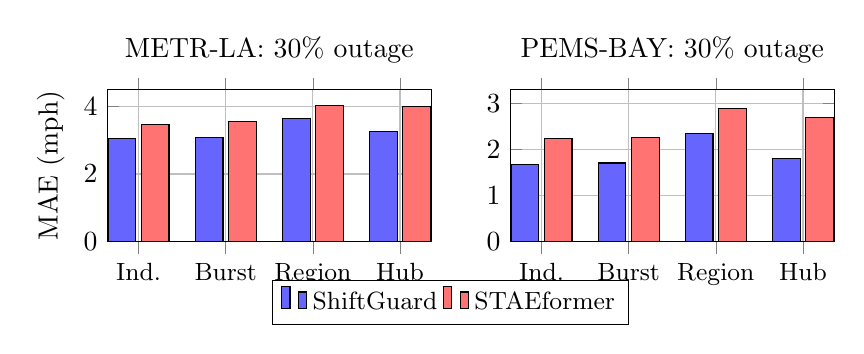
\begin{tikzpicture}
    \begin{groupplot}[
      group style={group size=2 by 1,horizontal sep=1.0cm},
      ybar,width=0.47\textwidth,height=0.29\textwidth,
      symbolic x coords={Ind.,Burst,Region,Hub},xtick=data,
      xticklabel style={font=\small},ymin=0,grid=major,enlarge x limits=0.12,
      legend style={font=\small,at={(1.06,-0.25)},anchor=north,legend columns=2}]
      \nextgroupplot[title={METR-LA: 30\% outage},ylabel={MAE (mph)},ymax=4.5]
        \addplot[fill=blue!60] coordinates {(Ind.,3.056) (Burst,3.076) (Region,3.632) (Hub,3.261)};
        \addlegendentry{ShiftGuard}
        \addplot[fill=red!55] coordinates {(Ind.,3.474) (Burst,3.541) (Region,4.027) (Hub,4.000)};
        \addlegendentry{STAEformer}
      \nextgroupplot[title={PEMS-BAY: 30\% outage},ymax=3.3]
        \addplot[fill=blue!60] coordinates {(Ind.,1.670) (Burst,1.707) (Region,2.348) (Hub,1.797)};
        \addplot[fill=red!55] coordinates {(Ind.,2.231) (Burst,2.250) (Region,2.893) (Hub,2.690)};
    \end{groupplot}
  \end{tikzpicture}
  \caption{Outage-family comparison at 30\% severity, averaged over five seeds
  (Ind. = independent loss).
  Contiguous-region failure is the hardest condition for ShiftGuard, whereas
  hub failure particularly harms STAEformer on PEMS-BAY.}
  \label{fig:outage-family}
\end{figure*}

Failure geometry further qualifies the result. At 30\% severity, ShiftGuard
reduces STAEformer MAE by 0.395--0.739 mph on METR-LA and by 0.543--0.893 mph on
PEMS-BAY, with the largest reduction for hub loss on both datasets.
Contiguous-region loss remains the hardest condition in absolute terms because
it removes an internally coherent subgraph and leaves fewer informative
boundaries from which to infer missing states, but the advantage over
STAEformer persists there (0.395 and 0.545 mph), although region outages never
occur during training. Hub loss disrupts STAEformer's global spatial
interaction more strongly, while ShiftGuard can fall back on its local residual
path and training-time node outages.

\subsection{Recipe versus architecture}
\label{sec:fair-comparison}
Each baseline is compared in three forms, as published, with outage augmentation,
and with outage augmentation plus the Laplace output, against ShiftGuard on the
timelines of Section~\ref{sec:deployment-protocol}.
\pending{Table from deployment\_summary.csv. Report (i) how much MAE each baseline
recovers from augmentation alone; (ii) ShiftGuard's margin over augmented
STAEformer with crossed intervals; (iii) whether the Laplace variants reach
ShiftGuard-like retention and failure. If a recipe-equipped baseline beats
ShiftGuard, state that the recipe, not the reference model, is the contribution,
and lead with the best recipe-equipped backbone.}

\subsection{Natural sensor missingness}
\label{sec:natural-missingness}
Synthetic masks cannot by themselves show that the protocol reflects field
failures. METR-LA provides a partial check, because 8.1\% of its readings are
missing and 98.3\% of test origins contain at least one missing input. In this
analysis no synthetic mask is applied: test origins are grouped by their own
input-missingness pattern, and every model uses the same prequential
calibration and risk controller as in the stress protocol. Two real failure
types dominate. Partial outages, in which individual sensors are silent while
the rest of the network reports, affect 5,832 origins and consist mostly of
sensors that are missing for the whole input window. Network-wide dropouts, in
which at least 90\% of sensors are missing at some input step, affect 898
origins and account for about 80\% of missing input cells.
Table~\ref{tab:natural-missingness} reports the results.

Real missingness is milder than the 30\% stress scenarios, and average
accuracy differences are correspondingly small. Over all test origins,
ShiftGuard's MAE is 3.004 mph against 3.032 mph for STAEformer. ShiftGuard is
0.021 mph better on origins with at most 5\% missing inputs, 0.041 mph better
above 5\%, and 0.068 mph better during network-wide dropouts. The differences
concentrate on silent sensors. For cells whose sensor reported nothing during
the input window but whose target was observed, ShiftGuard's error is 5.18 and
5.56 mph in the two partial-outage strata, compared with 5.78 and 7.08 mph for
STAEformer and 6.67--10.22 mph for the graph and identity baselines. The legacy
model with reliability weighting is worse on these cells (5.44 and 6.10 mph),
consistent with the validation-based model selection. For the legacy model,
training without outage augmentation raised these errors further to 5.65 and
6.30 mph, so augmentation accounts for part, but not all, of the gap; the rest
is associated with supplying the observation mask as an input.
\pending{Replace the legacy no-augmentation comparison with the reference
model's no-augmentation ablation once trained.}

ShiftGuard's 90\% intervals keep coverage between 0.889 and 0.900 in every
stratum, whereas STAEformer and the graph baselines fall to 0.874--0.878 when
more than 5\% of inputs are missing. Over all origins, ShiftGuard retains
98.8\% of forecasts with 5.1\% accepted-origin failure, compared with 79.8\% and
6.2\% for STAEformer. The analysis also exposes a failure mode that the synthetic
protocol does not. During network-wide dropouts, every model exceeds the 10\%
risk target among accepted origins: ShiftGuard reaches 14.9\% and STAEformer
21.3\%, because the controller still accepts 95\% and 90\% of these origins.
Such dropouts form 13\% of test origins, so the pooled prequential threshold is
dominated by ordinary conditions. In deployment, the controller should
therefore be paired with an explicit fallback when most of the network is
silent; we report this as an open failure mode rather than a solved case.
\pending{Add the outage-augmented baselines to this paragraph once their five
seeds are complete.}
\begin{table}[t]
  \centering
  \caption{METR-LA test origins grouped by their own input missingness, with
  no synthetic outage applied; mean over five seeds. Dead-sensor MAE is
  computed on cells whose sensor was missing for the whole input window but
  whose target was observed. Failure rate is the share of accepted origins
  with mean absolute error above 5 mph.}
  \label{tab:natural-missingness}
  \resizebox{\columnwidth}{!}{\begin{tabular}{llrlrrrrr}
\toprule
Dataset & Input missingness & Origins & Model & MAE & Dead-sensor MAE & PI coverage & Retained & Failure rate \\
\midrule
METR-LA & Complete inputs & 114 & ShiftGuard w/o outage aug. & 2.934 & -- & 0.896 & 1.000 & 0.018 \\
METR-LA & Complete inputs & 114 & ShiftGuard & 2.945 & -- & 0.898 & 1.000 & 0.018 \\
METR-LA & Complete inputs & 114 & STAEformer & 3.011 & -- & 0.899 & 1.000 & 0.019 \\
METR-LA & Complete inputs & 114 & DCRNN & 3.056 & -- & 0.905 & 0.000 & -- \\
METR-LA & Complete inputs & 114 & STID & 3.063 & -- & 0.906 & 0.000 & -- \\
METR-LA & Complete inputs & 114 & Graph WaveNet & 3.153 & -- & 0.904 & 0.000 & -- \\
METR-LA & Dead sensors, <=5\% missing & 5014 & ShiftGuard w/o outage aug. & 2.928 & 5.652 & 0.901 & 0.995 & 0.042 \\
METR-LA & Dead sensors, <=5\% missing & 5014 & STAEformer & 2.961 & 5.778 & 0.901 & 0.750 & 0.047 \\
METR-LA & Dead sensors, <=5\% missing & 5014 & ShiftGuard & 2.968 & 5.440 & 0.901 & 0.988 & 0.043 \\
METR-LA & Dead sensors, <=5\% missing & 5014 & DCRNN & 3.152 & 6.927 & 0.902 & 0.105 & 0.053 \\
METR-LA & Dead sensors, <=5\% missing & 5014 & STID & 3.191 & 7.310 & 0.902 & 0.070 & 0.093 \\
METR-LA & Dead sensors, <=5\% missing & 5014 & Graph WaveNet & 3.194 & 6.667 & 0.902 & 0.092 & 0.069 \\
METR-LA & Dead sensors, >5\% missing & 818 & ShiftGuard w/o outage aug. & 3.274 & 6.297 & 0.898 & 0.999 & 0.074 \\
METR-LA & Dead sensors, >5\% missing & 818 & ShiftGuard & 3.309 & 6.096 & 0.899 & 0.984 & 0.074 \\
METR-LA & Dead sensors, >5\% missing & 818 & STAEformer & 3.312 & 7.083 & 0.878 & 0.954 & 0.080 \\
METR-LA & Dead sensors, >5\% missing & 818 & DCRNN & 3.587 & 9.053 & 0.876 & 0.334 & 0.127 \\
METR-LA & Dead sensors, >5\% missing & 818 & STID & 3.597 & 10.221 & 0.877 & 0.249 & 0.181 \\
METR-LA & Dead sensors, >5\% missing & 818 & Graph WaveNet & 3.638 & 8.681 & 0.874 & 0.334 & 0.149 \\
METR-LA & Network-wide dropout & 898 & ShiftGuard & 3.396 & 4.832 & 0.887 & 0.950 & 0.173 \\
METR-LA & Network-wide dropout & 898 & ShiftGuard w/o outage aug. & 3.439 & 4.812 & 0.889 & 0.937 & 0.181 \\
METR-LA & Network-wide dropout & 898 & STAEformer & 3.450 & 4.869 & 0.889 & 0.898 & 0.213 \\
METR-LA & Network-wide dropout & 898 & STID & 3.836 & 5.071 & 0.886 & 0.014 & 0.323 \\
METR-LA & Network-wide dropout & 898 & Graph WaveNet & 3.881 & 5.356 & 0.883 & 0.069 & 0.551 \\
METR-LA & Network-wide dropout & 898 & DCRNN & 3.962 & 5.396 & 0.879 & 0.123 & 0.538 \\
\bottomrule
\end{tabular}
}
\end{table}

\subsection{Selective forecasting, ablation, and efficiency}
At 30\% severity, prequential risk control reduces accepted-origin failure on
METR-LA from 11\% without abstention to 7\%, while retaining 91\% of forecasts.
On PEMS-BAY it reduces failure from 3\% to 2\% at 98\% retention. Static
calibration fails under drift on METR-LA (11\% failure despite almost full
retention), supporting online updates. Table~\ref{tab:calibration} reports all registered
calibration controls.
\begin{table}[t]
  \centering
  \caption{Calibration and selection controls at 30\% outage severity,
  averaged over non-clean families and five seeds.}
  \label{tab:calibration}
  \resizebox{\columnwidth}{!}{\begin{tabular}{lllrrr}
\toprule
Dataset & Calibration & Selection & PI coverage & Retained & Failure rate \\
\midrule
METR-LA & global-prequential & risk & 0.899 & 0.912 & 0.072 \\
METR-LA & group-prequential & all & 0.899 & 1.000 & 0.112 \\
METR-LA & group-prequential & risk & 0.899 & 0.906 & 0.072 \\
METR-LA & group-static & risk & 0.899 & 0.998 & 0.112 \\
PEMS-BAY & global-prequential & risk & 0.898 & 0.970 & 0.019 \\
PEMS-BAY & group-prequential & all & 0.898 & 1.000 & 0.027 \\
PEMS-BAY & group-prequential & risk & 0.898 & 0.979 & 0.019 \\
PEMS-BAY & group-static & risk & 0.886 & 0.982 & 0.023 \\
\bottomrule
\end{tabular}
}
\end{table}

\begin{figure*}[t]
  \centering
  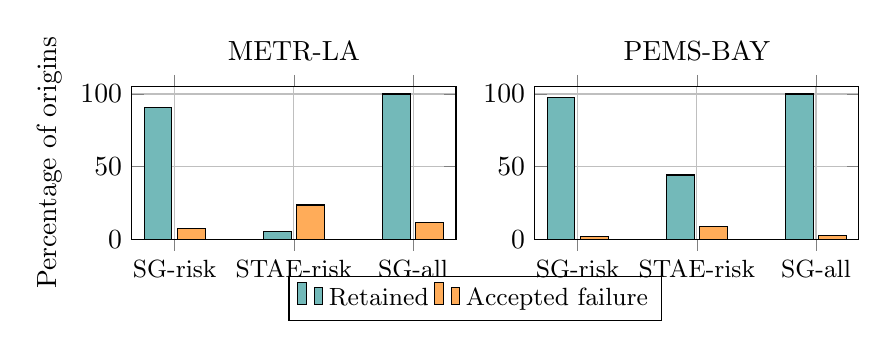
\begin{tikzpicture}
    \begin{groupplot}[
      group style={group size=2 by 1,horizontal sep=1.0cm},
      ybar,width=0.47\textwidth,height=0.29\textwidth,
      symbolic x coords={SG-risk,STAE-risk,SG-all},xtick=data,
      xticklabel style={font=\small},ymin=0,ymax=105,grid=major,enlarge x limits=0.18,
      ylabel={Percentage of origins},
      legend style={font=\small,at={(1.06,-0.24)},anchor=north,legend columns=2}]
      \nextgroupplot[title={METR-LA}]
        \addplot[fill=teal!55] coordinates {(SG-risk,90.6) (STAE-risk,5.5) (SG-all,100.0)};
        \addlegendentry{Retained}
        \addplot[fill=orange!65] coordinates {(SG-risk,7.2) (STAE-risk,23.5) (SG-all,11.2)};
        \addlegendentry{Accepted failure}
      \nextgroupplot[title={PEMS-BAY},ylabel={}]
        \addplot[fill=teal!55] coordinates {(SG-risk,97.9) (STAE-risk,44.2) (SG-all,100.0)};
        \addplot[fill=orange!65] coordinates {(SG-risk,1.9) (STAE-risk,8.5) (SG-all,2.7)};
    \end{groupplot}
  \end{tikzpicture}
  \caption{Operational selection outcomes at 30\% severity. SG-risk denotes
  ShiftGuard with the registered controller; STAE-risk applies the same
  controller to STAEformer; SG-all releases every forecast. High retention is
  useful only when accepted-origin failure also remains low.
  Legacy protocol. STAE-risk uses a point-only STAEformer, whose intervals carry
  little origin-level information; Section~\ref{sec:fair-comparison} gives the
  recipe-matched comparison.}
  \label{fig:selection-outcomes}
\end{figure*}

Global-prequential and group-prequential ShiftGuard have nearly identical
marginal coverage and operational results at the displayed precision. Static
group calibration performs poorly on METR-LA: it retains 99.9\% of origins but
fails on 11.2\% of them, no better than releasing every forecast. On the more
stationary PEMS-BAY the gap is smaller: static calibration retains 98.2\% with
2.3\% failure and 0.886 coverage, whereas prequential grouping retains 97.9\%
with 1.9\% failure and 0.898 coverage. The value of rolling adaptation is
therefore strongest on the dataset with more native missingness and transition
activity.

\pending{Summarize the reference model's ablations under the deployment
scenarios, including the no-mask-input ablation.} In the legacy model (Table~\ref{tab:ablation-legacy}),
removing structured augmentation increased MAE by 0.306 mph on METR-LA and 0.703
mph on PEMS-BAY, independent masking alone lost 0.098 and 0.220 mph, removing
reliability weighting improved MAE by 0.143 and 0.067 mph, and removing the
router had a small favorable effect. The ablations therefore identify structured augmentation as the
effective component of the reference model and falsifies the stronger claim
that every proposed mechanism is necessary. Together with
Section~\ref{sec:fair-comparison}, this is why the paper's claims are made at
the level of the recipe rather than the architecture.
\begin{table}[t]
  \centering
  \caption{Ablations of the legacy ShiftGuard model (with reliability
  weighting) at 30\% severity. These test results motivated, but did not
  decide, the reference-model selection in
  Section~\ref{sec:reference-selection}.}
  \label{tab:ablation-legacy}
  \IfFileExists{generated_ablation_legacy.tex}{%
    \resizebox{0.86\columnwidth}{!}{\begin{tabular}{llrrrr}
\toprule
Dataset & Variant & MAE & AURC & Retained & Seeds \\
\midrule
METR-LA & Legacy ShiftGuard (reference + reliability weighting) & 3.399 & 2.400 & 0.864 & 5 \\
METR-LA & Adaptive graph only & 3.319 & 2.362 & 0.884 & 5 \\
METR-LA & Independent masking only & 3.496 & 2.508 & 0.820 & 5 \\
METR-LA & No outage augmentation & 3.705 & 2.657 & 0.740 & 5 \\
METR-LA & No reliability weighting (= reference) & 3.256 & 2.339 & 0.906 & 5 \\
METR-LA & No regime router & 3.372 & 2.392 & 0.872 & 5 \\
METR-LA & Static graph only & 3.469 & 2.448 & 0.841 & 5 \\
PEMS-BAY & Legacy ShiftGuard (reference + reliability weighting) & 1.948 & 1.130 & 0.978 & 5 \\
PEMS-BAY & Adaptive graph only & 1.884 & 1.108 & 0.983 & 5 \\
PEMS-BAY & Independent masking only & 2.168 & 1.204 & 0.935 & 5 \\
PEMS-BAY & No outage augmentation & 2.651 & 1.735 & 0.917 & 5 \\
PEMS-BAY & No reliability weighting (= reference) & 1.881 & 1.098 & 0.979 & 5 \\
PEMS-BAY & No regime router & 1.927 & 1.115 & 0.977 & 5 \\
PEMS-BAY & Static graph only & 2.056 & 1.238 & 0.952 & 5 \\
\bottomrule
\end{tabular}
}}{%
    \pending{generated by scripts/aggregate\_results.py}}
\end{table}

ShiftGuard uses 89k/100k parameters on METR-LA/PEMS-BAY versus
1.26M/1.37M for STAEformer; disabling reliability weighting does not change
the parameter count. \pending{Re-measure on an idle GPU; legacy-model values:}
its batch-one latency is 2.30/2.43 ms, and its
batch-eight throughput is 3567/3335 samples s$^{-1}$, compared with 503/269
for STAEformer on the same RTX 5060 Laptop GPU. Table~\ref{tab:efficiency}
reports the principal local efficiency controls.
\begin{table}[!htbp]
  \centering
  \caption{Local GPU efficiency; latency uses batch one and throughput/memory
  use batch eight. FLOPs are profiler-observed operations per sample.}
  \label{tab:efficiency}
  \resizebox{0.90\columnwidth}{!}{\begin{tabular}{llrrrrr}
\toprule
Dataset & Model & Parameters & FLOPs/sample & Latency B1 (ms) & Throughput B8 & Memory B8 (MiB) \\
\midrule
METR-LA & DCRNN & 63372 & 845712576.00 & 7.97 & 1052.04 & 38.27 \\
METR-LA & Graph WaveNet & 22744 & 189736407.00 & 1.86 & 7136.17 & 47.52 \\
METR-LA & STID & 41996 & 4040706.00 & 0.47 & 16822.62 & 34.97 \\
METR-LA & STAEformer & 1258932 & 6080479272.00 & 2.62 & 502.59 & 180.93 \\
METR-LA & ShiftGuard & 89012 & 38541287.00 & 2.30 & 3567.45 & 36.95 \\
PEMS-BAY & DCRNN & 63372 & 1806417600.00 & 7.47 & 1045.04 & 42.00 \\
PEMS-BAY & Graph WaveNet & 25104 & 387135775.00 & 1.50 & 6071.88 & 57.62 \\
PEMS-BAY & STID & 49548 & 6344066.00 & 0.49 & 16769.73 & 36.60 \\
PEMS-BAY & STAEformer & 1372212 & 10386051000.00 & 3.68 & 268.54 & 319.69 \\
PEMS-BAY & ShiftGuard & 100340 & 76656703.00 & 2.43 & 3335.28 & 42.18 \\
\bottomrule
\end{tabular}
}
\end{table}

\begin{figure}[!htbp]
  \centering
  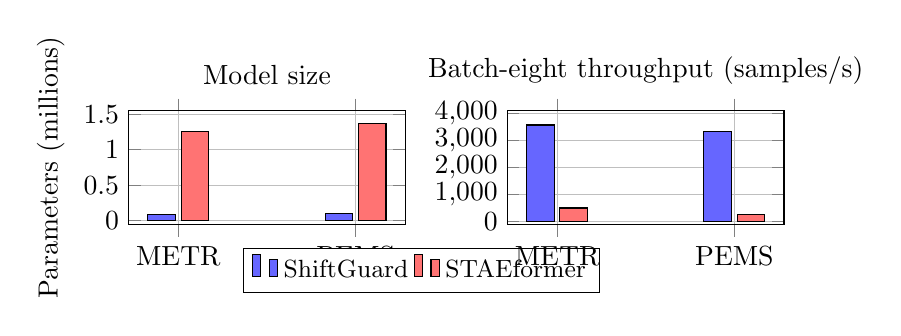
\begin{tikzpicture}
    \begin{groupplot}[
      group style={group size=2 by 1,horizontal sep=1.3cm},
      ybar,width=0.42\textwidth,height=0.25\textwidth,
      symbolic x coords={METR,PEMS},xtick=data,grid=major,enlarge x limits=0.28,
      legend style={font=\small,at={(1.06,-0.20)},anchor=north,legend columns=2}]
      \nextgroupplot[title={Model size},ylabel={Parameters (millions)},ymax=1.55]
        \addplot[fill=blue!60] coordinates {(METR,0.089) (PEMS,0.100)};
        \addlegendentry{ShiftGuard}
        \addplot[fill=red!55] coordinates {(METR,1.259) (PEMS,1.372)};
        \addlegendentry{STAEformer}
      \nextgroupplot[title={Batch-eight throughput (samples/s)},ylabel={},ymax=4100]
        \addplot[fill=blue!60] coordinates {(METR,3567) (PEMS,3335)};
        \addplot[fill=red!55] coordinates {(METR,503) (PEMS,269)};
    \end{groupplot}
  \end{tikzpicture}
  \caption{Efficiency comparison with the strongest local transformer.
  \pending{throughput bars show the legacy model until re-measured.}
  ShiftGuard uses 13.7--14.1 times fewer parameters and provides 7.1--12.4
  times higher batch-eight throughput on the disclosed GPU.}
  \label{fig:efficiency-tradeoff}
\end{figure}

Figure~\ref{fig:efficiency-tradeoff} complements the error tables with resource
cost. ShiftGuard is roughly fourteen times smaller than STAEformer and uses
about one fifth to one eighth of its batch-eight allocated GPU memory. The
advantage is especially large on PEMS-BAY, where the spatial attention axis
contains 325 sensors. STID and Graph WaveNet remain faster than ShiftGuard in
the local benchmark, so ShiftGuard is not an absolute efficiency SOTA. Its
claim is instead a favorable joint operating point: substantially lower outage
error than those compact baselines while using far fewer resources.

\section{Discussion}
\subsection{Answers to the research questions}
\pending{Rewrite these answers from Section~\ref{sec:deployment-results}. The
figures below come from the legacy stress protocol, and any that survive must be
labelled as such.}

\textbf{RQ1: point robustness.} The results support the value of
structured-outage training on both datasets. Averaged over 20 non-clean
family--severity scenarios, ShiftGuard reduces MAE relative to the strongest
local transformer by 0.476 mph on METR-LA and 0.617 mph on PEMS-BAY. The crossed
seed--scenario bootstrap intervals exclude zero, and the separation grows with
severity in Figure~\ref{fig:robustness-severity}. The effect is not confined to
independent masking: Figure~\ref{fig:outage-family} shows an advantage in every
registered outage family, including the region and hub geometries that are
held out from training. Region failure remains the hardest condition in
absolute terms, because a connected missing set removes both local history and
the most useful neighbors.

\textbf{RQ2: subgroup interval reliability.} At 30\% severity, ShiftGuard's
90\% intervals achieve about 0.898 marginal coverage on both datasets. More
importantly, worst node--horizon coverage is 0.830 versus 0.816 for
STAEformer on METR-LA and 0.852 versus 0.834 on PEMS-BAY, while worst-regime
coverage is 0.887 versus 0.809 and 0.876 versus 0.701. The PEMS-BAY
difference is operationally meaningful: STAEformer's 0.701 worst-regime
coverage means that a marginally acceptable interval can fail badly for a
particular traffic state. Group-prequential calibration does not make every
subgroup exactly 90\%; finite calibration samples, temporal dependence, and
abrupt transitions prevent that interpretation. It does, however, reduce the
disparity relative to the strongest comparator.

\textbf{RQ3: selective risk.} The origin-level controller provides the clearest
deployment advantage. The STAEformer figures below use a point-only model,
whose origin-level interval widths carry little ranking information, so they
bound the benefit of a learned scale rather than of the architecture;. On METR-LA, ShiftGuard retains 90.6\% of forecasts with a
7.2\% empirical failure rate, compared with 5.5\% retention and 23.5\% failure
for STAEformer under the same selection rule. On PEMS-BAY it retains 97.9\%
with 1.9\% failure, versus 44.2\% and 8.5\%. Releasing every ShiftGuard forecast
raises failure to 11.2\% and 2.7\%, respectively. The PEMS-BAY all-forecast rate
is already below the 10\% target, yet risk control still removes a small harmful
tail. On METR-LA, abstention materially changes whether the target is met. AURC
improvements of 1.51 and 1.28 show that the interval-derived score ranks
high-error origins better across the full retention continuum, not only at one
threshold.

\textbf{RQ4: recipe versus architecture.} Two lines of evidence narrow the
explanation. In the legacy model, removing structured augmentation increased
30\%-severity MAE by 0.306 mph on METR-LA and 0.703 mph on PEMS-BAY, whereas
removing reliability-weighted propagation improved MAE by 0.143 and 0.067 mph;
validation data then confirmed the simpler reference model.
\pending{Reference-model ablations and the recipe-matched comparison under the
deployment scenarios.} The robustness gain is
therefore attributed to the training distribution, calibrated scale output,
and decision layer, not to every architectural module. ShiftGuard remains a
useful carrier of the recipe because it is computationally cheap: 89k/100k
parameters and, \pending{re-measure; legacy values:} 37/42 MiB batch-eight
peak allocated memory and 7.1 and 12.4 times the throughput of the local
STAEformer on METR-LA and PEMS-BAY.

\subsection{Why clean accuracy and deployment reliability disagree}
The clean results illustrate why average benchmark rankings should not be
treated as deployment rankings. STAEformer and ShiftGuard are indistinguishable
on METR-LA at the tested resolution, while STAEformer is significantly better
on clean PEMS-BAY. Under outage, the relationship reverses. STAEformer's
adaptive embeddings and attention are highly effective when all node histories
are present, but the model was not optimized to interpret an explicit failure
mask or to reconstruct information from structured partial histories.
ShiftGuard sacrifices a small amount of clean PEMS-BAY accuracy in exchange for
a training distribution that covers missingness. This is a conventional
robustness trade-off rather than evidence that either model is universally
superior.

For an ITS operator, the preferred model depends on the cost function. If
sensors are centrally managed, outages are negligible, and every prediction
must be released, STAEformer may be preferred on PEMS-BAY. If communication
loss, maintenance, or corridor failure is plausible and the controller can fall
back to a safe policy, ShiftGuard offers a more useful risk--coverage profile.
This distinction motivates reporting clean accuracy, stressed accuracy,
calibration, selection, and resource cost as separate axes rather than
collapsing them into one leaderboard.

\subsection{Statistical interpretation}
The hierarchical bootstrap resamples both seeds and outage scenarios, matching
the two principal replicated axes. Its confidence intervals support a stable
average robustness effect. The seed-level Wilcoxon tests remain non-significant
after Holm correction because five seeds permit only a coarse attainable
two-sided rank-test resolution. We therefore do not use the bootstrap interval
to claim that the adjusted rank test is significant, nor do we reinterpret
non-significance as equivalence. Both are reported because they answer
different questions: the interval estimates the effect under hierarchical
resampling, whereas the rank test provides a conservative seed-level check.

The risk certificate has an equally important qualification. The exact
binomial upper bound assumes that accepted-origin failures in the certification
sample behave as i.i.d. Bernoulli trials. Traffic origins overlap and are
temporally dependent, so that assumption is an approximation. Disjoint
construction and certification samples prevent direct outcome reuse, and the
prequential order prevents future leakage, but neither operation proves
independence. Accordingly, the paper calls the observed quantities empirical
prequential coverage and failure. A stronger time-series certificate would
require mixing assumptions, blockwise methods, martingale bounds, or online
guarantees explicitly designed for dependent sequences.

\subsection{Threats to validity and generalizability}
Several limitations bound the claims. First, METR-LA and PEMS-BAY are freeway
speed datasets from 2012 and 2017. They do not represent signalized urban
arterials, multimodal demand, weather extremes, special events, or contemporary
connected-vehicle telemetry. Second, the correlation graph is learned from
training data rather than a verified directed road topology. Correlation can
connect sensors that co-vary because of common demand but lack a direct physical
link; it also makes the region and hub stress families properties of the proxy
graph. Third, synthetic outages are reproducible and controllable but cannot
capture every field failure mechanism. Real outages may co-occur with incidents,
produce delayed or biased readings rather than complete absence, and have
repair dynamics not represented here. Because the training and test outage
generators are designed by the same authors, part of any robustness gain could
reflect matched assumptions; holding out region and hub geometries mitigates
but does not remove this risk. No live outage logs or field deployment are
evaluated, so the results establish robustness under a controlled and
reproducible protocol, not operational dependability. Trace replay improves
realism but remains retrospective: traces come from one network and are
transplanted to PEMS-BAY without preserving physical sensor identity. The
legacy stress results additionally carry the defects described in
Section~\ref{sec:legacy-protocol}, and neither test set contains congested
origins, so behavior under sustained network-wide congestion is untested.
The natural-missingness analysis in Section~\ref{sec:natural-missingness}
is a partial check on real failure patterns. It shows smaller average
differences than the synthetic protocol, a consistent advantage on silent
sensors, and a failure mode during network-wide dropouts that synthetic
outages did not reveal. It covers one dataset and the outage types that
happened to occur in its test period.

Fourth, locally reproduced graph baselines are protocol-matched compact
implementations, not bitwise reproductions of every official repository.
Literature-reported values are therefore kept in a separate contextual table
and never enter paired significance claims. Recipe-matched baselines reuse
their original hyperparameters; tuning them specifically for masked inputs
could narrow differences further. Fifth, hyperparameters were selected
under a finite validation budget and may favor neither model optimally. Sixth,
the operational failure threshold of 5 mph and risk limit of 10\% are plausible
research choices, not universal policy standards. A traffic management center
must select them from the consequences of false alarms, unsafe actuation, and
fallback availability. Finally, all experiments use one GPU platform; latency
rankings can change with compilation, precision, batch size, and edge hardware.

Despite these constraints, the design offers useful internal validity. Both
datasets share the same preprocessing and split logic; masks are deterministic
and paired across models; five seeds are used for stochastic models; test
targets never tune the predictor or controller; all tables are generated from
machine-readable artifacts; and negative ablation findings are retained. These
controls make the central conclusion reproducible within the declared scope.

\section{Future work}
The first priority is prospective validation. A deployment study should ingest
live detector health logs, communication alarms, maintenance records, weather,
and incident annotations, then evaluate forecasts before outcomes are known.
Such data would reveal whether the four synthetic outage families span real
failure geometry and whether risk control triggers early enough for an operator
to switch to a safe fallback. Evaluation should expand to signalized urban
networks, arterial travel times, traffic flow and occupancy, and geographically
distinct cities. Cross-city transfer would test whether structured augmentation
learns a general robustness principle or benchmark-specific correlations.

The second priority is stronger dependent-data inference. Block conformal,
weighted conformal, martingale, and change-point-aware methods could replace the
i.i.d. binomial approximation. A promising design would jointly adapt the
rolling window, subgroup shrinkage, and risk threshold according to detected
regime duration while preserving anytime validity. Hierarchical calibration
could pool information among nearby sensors without allowing large groups to
hide minority undercoverage. Conditional coverage remains impossible without
additional assumptions in full generality, so future work should state the
precise dependence or smoothness structure under which stronger guarantees are
obtained.

Third, the negative ablations and the recipe-matched comparison suggest that
effort is better spent on the training distribution and decision layer than on
new spatial modules. A lean reference model without the router and
reliability-weighted propagation, with the parameter budget reallocated to a
stronger mask-aware temporal encoder, may improve both clean and stressed
accuracy. Learned corruption generators could approximate empirical
failure logs, while adversarial graph outages could locate worst-case vulnerable
subnetworks. Any such extension should retain the current fixed-mask paired
evaluation to separate a genuinely stronger model from a more favorable stress
sample.

Fourth, decision quality should be connected to transportation outcomes.
Forecast MAE and a 5 mph tensor threshold are proxies. Simulation could measure
travel time, queue spillback, ramp-metering stability, incident response delay,
or regret of the downstream control action. Abstention could select among
fallbacks rather than return a binary rejection: persistence, historical
profiles, a physics-based model, human review, or a neighboring data source may
have different costs. Multi-objective risk control could then balance safety,
coverage, latency, and energy use.

Finally, uncertainty should be decomposed and communicated. Deep ensembles,
Bayesian approximations, and conformalized quantile models could distinguish
data uncertainty from model uncertainty, while attribution maps could explain
which unavailable sensors caused abstention. Edge deployment studies should
include quantization, mixed precision, pruning, and end-to-end communication
latency. These directions would move the present benchmark contribution toward
a certifiable, interpretable, and maintainable ITS service.

\section{Conclusion}
This study reframes short-term network traffic forecasting as a joint point,
interval, and selective-decision problem under compound traffic-regime and
sensor-availability shift, and argues that reliability under that shift is
mainly a property of training, calibration, and gating. The proposed recipe
combines structured-outage augmentation, a Laplace median--scale output,
rolling node--horizon conformalization, and an origin-level act/abstain rule.
Evidence gating extends it to silent sensors. The accompanying deployment-feasible
protocol evaluates outage timelines that persist across origins, including
replayed real availability traces, with calibration limited to information
available in deployment and abstention scored against a real fallback.

The empirical conclusion is specific. ShiftGuard, the compact reference model,
is not a clean-data state of the art: it is 0.03 mph better than STAEformer on
clean METR-LA and 0.013 mph worse on clean PEMS-BAY. \pending{Deployment results
and the recipe-transfer outcome; state ShiftGuard's role accordingly.} On METR-LA's
naturally missing inputs the average gain largely disappears, but the advantage
on silent sensors and the stability of interval coverage persist. Legacy ablations
attribute the point gain to outage-structured augmentation rather than to
reliability-weighted propagation or routing, which validation data led us to
remove.

The work does not claim a new architecture, unconditional coverage under
temporal dependence, or operational dependability established by field
deployment. Within its declared scope, it demonstrates that asking \emph{when
not to trust a traffic forecast} changes both model ranking and evaluation
practice, and it provides a protocol and recipe that other forecasters can
adopt. Future progress should validate that conclusion on prospective outage
logs, newer urban networks, dependent-data certificates, and downstream
traffic-control outcomes.

\section*{Data and code availability}
The source code, experiment configurations, fixed seeds, stress-mask generators,
training and evaluation scripts, and table-generation utilities are openly
available at \url{https://github.com/shishirbit/ShiftGuard-ITS}. Large generated
checkpoints and prediction tensors are excluded from version control. The
METR-LA and PEMS-BAY benchmark files are available through the official DCRNN
data-preparation repository at \url{https://github.com/liyaguang/DCRNN#data-preparation}
and its linked dataset archive at
\url{https://drive.google.com/drive/folders/10FOTa6HXPqX8Pf5WRoRwcFnW9BrNZEIX}.
PEMS-BAY originates from the California Department of Transportation Performance
Measurement System (PeMS), \url{https://pems.dot.ca.gov/}. The raw benchmark
files are not redistributed in this repository.

\bibliographystyle{elsarticle-num}
\bibliography{references}
\end{document}
